% !TEX program = xelatex

% === Biên dịch bằng XeLaTeX ===
% (TeX -> XeLaTeX) để hỗ trợ tiếng Việt + Times New Roman
\documentclass[13pt,a4paper]{extreport}
% --- Ngôn ngữ & font ---
\usepackage{fontspec}
\usepackage{polyglossia}
\setmainlanguage{vietnamese} % Ngôn ngữ chính: tiếng Việt
\setotherlanguage{english}   % Ngôn ngữ phụ: tiếng Anh
\setmainfont{Times New Roman}
\setsansfont{Times New Roman}

% Nếu có công thức toán hoặc ký tự đặc biệt trong toán học:
\usepackage{amsmath, amssymb, amsfonts} % Toán học
\usepackage{unicode-math}
\setmathfont{XITS Math}

\usepackage{fontawesome5} % Cung cấp các biểu tượng như \faCheck, \faTimes
\usepackage{textcomp}

%Thư mục project
\usepackage{dirtree}
\usepackage{needspace}

% --- Ký hiệu tiện dụng ---
\newcommand{\concat}{\mathbin{\|}} % phép nối chuỗi (concatenation)
 % Ký hiệu như °, €, ™

% --- Giấy & lề theo quy định TDTU ---
\usepackage{geometry}
\geometry{paper=a4paper, top=3.5cm, bottom=3cm, left=3.5cm, right=2cm, headheight=25pt}
\setlength{\headsep}{10pt}

% --- Giãn dòng 1.5 ---
\usepackage{setspace}
\onehalfspacing

% --- Đồ hoạ, bảng biểu, mã nguồn ---
\usepackage{graphicx}
\usepackage{caption}
\usepackage{subcaption}
\usepackage{float}
\usepackage{booktabs}
\usepackage{longtable}
\usepackage{tabularx}
\usepackage{array}
\usepackage{multirow}
\usepackage{listings}
\lstset{basicstyle=\ttfamily\small, breaklines=true, frame=single}

% --- Màu sắc (một lần) ---
\usepackage[table]{xcolor}
\usepackage[T1]{fontenc}
\usepackage{inconsolata} % monospace đẹp (tuỳ chọn)
\usepackage{xcolor}
\usepackage{minted}

% Style chung cho code
\setminted{
  fontsize=\small,
  breaklines=true,
  breakanywhere=true,
  autogobble=true,
  tabsize=4,
  linenos=true,
  numbersep=6pt,
  frame=lines,
  framesep=3mm
}

% --- Toán học (nếu cần) ---
% (đã nạp amsmath/amssymb ở phần trên)

% --- Sơ đồ (TikZ) ---
\usepackage{tikz}
\usetikzlibrary{shapes.geometric, arrows.meta, positioning, fit, calc, backgrounds, shadows, shadows.blur, decorations.pathreplacing}

% --- Liên kết ---
\usepackage{csquotes} % cần cho biblatex
\usepackage[hyphens]{url} % Cho phép ngắt dòng URL tại dấu gạch nối
% --- Tiêu đề chương/mục & Mục lục ---
\usepackage{tocloft}
\setcounter{tocdepth}{2}

\setlength{\headsep}{10pt}
% Hiển thị "CHƯƠNG" trước số chương và trong Mục lục
\addto\captionsvietnamese{\renewcommand{\chaptername}{CHƯƠNG}}
\renewcommand{\cftchappresnum}{\chaptername\ }
\renewcommand{\cftchapnumwidth}{7em}
\renewcommand{\cftchapaftersnum}{\hspace{0.5em}}
\renewcommand{\cftchapleader}{\cftdotfill{\cftdotsep}}

% Định dạng tiêu đề
\usepackage{titlesec}
% CHƯƠNG: 18pt (leading 20pt), đậm + căn giữa
\titleformat{\chapter}
  {\bfseries\fontsize{18pt}{20pt}\selectfont}
  {\chaptername\ \thechapter}{1em}{}
\titlespacing{\chapter}{0pt}{1.0\baselineskip}{1.0\baselineskip}
% \usepackage{etoolbox}
% \makeatletter
% \patchcmd{\@afterheading}{\@afterindentfalse}{\@afterindenttrue}{}{}
% \makeatother

% Xoay ngang trang
\usepackage{pdflscape}

\usepackage{microtype}

% Mục (section): 14pt (leading 16pt), đậm
\titleformat{\section}
  {\bfseries\fontsize{14pt}{16pt}\selectfont}
  {\thesection}{1em}{}
\titlespacing{\section}{0pt}{0.8\baselineskip}{0.8\baselineskip}

% Tiểu mục (subsection): 13pt (leading 15pt), đậm (thích thì thêm \itshape)
\titleformat{\subsection}
  {\bfseries\itshape\fontsize{13pt}{15pt}\selectfont}
  {\thesubsection}{1em}{}
\titlespacing{\subsection}{0pt}{0.6\baselineskip}{0.6\baselineskip}

\titleformat{\subsubsection}
  {\bfseries\fontsize{13pt}{15pt}\selectfont}
  {\thesubsubsection}{1em}{}
\titlespacing{\subsubsection}{0pt}{0.5\baselineskip}{0.5\baselineskip}

  
% --- Danh sách (không dùng quá 3 cấp) ---
\usepackage{enumitem}
\setlistdepth{4}
% Cấp 1: gạch ngang dài
\setlist[itemize,1]{label=--, left=0pt, itemsep=0.4em, topsep=0.4em}

% Cấp 2: dấu cộng (dùng math cho đẹp)
\setlist[itemize,2]{label={$+$}, left=1em, itemsep=0.3em, topsep=0.3em}

% Cấp 3: chấm tròn đen
\setlist[itemize,3]{label=\textbullet, left=2em, itemsep=0.2em, topsep=0.2em}


% --- Header & Footer: số trang giữa-đầu trang theo quy định ---
\usepackage{fancyhdr}
\pagestyle{fancy}
\fancyhf{}% xoá hết
\fancyhead[C]{\thepage} % số trang ở giữa phần đầu trang
\renewcommand{\headrulewidth}{0pt}
\renewcommand{\footrulewidth}{0pt}
% Trang kiểu "plain" (mặc định cho đầu chương) cũng đặt số ở đầu trang
\fancypagestyle{plain}{% áp cho các trang plain
\fancyhf{}
\fancyhead[C]{\thepage}
\renewcommand{\headrulewidth}{0pt}
}

% Tài liệu tham khảo
\usepackage[backend=biber,style=apa,citestyle=apa]{biblatex}
\addbibresource{references.bib}
\DeclareLanguageMapping{vietnamese}{vietnamese-apa}

% ===== Danh mục bảng biểu (List of Tables) =====
% Độ rộng vùng số (để canh thẳng hàng + đủ chỗ cho "Bảng 10.12" ...)
\setlength{\cfttabnumwidth}{4em} % tăng/giảm tuỳ bạn

% Khoảng cách giữa số và tên bảng
\renewcommand{\cfttabaftersnum}{\hspace{0.8em}} % tăng/giảm tuỳ bạn

% ===== Danh mục hình vẽ (List of Figures) =====
\setlength{\cftfignumwidth}{4em}
\renewcommand{\cftfigaftersnum}{\hspace{0.8em}}



% --- Liên kết (nên nạp sau biblatex để ổn định hơn) ---
\usepackage[hidelinks]{hyperref}
% --- Thụt đầu dòng ~1 tab ---
\usepackage{indentfirst}
\setlength{\parindent}{1.25cm}
\setlength{\parskip}{0pt}

\renewcommand{\figurename}{Hình}
\renewcommand{\tablename}{Bảng}

%============================================================
\begin{document}
% ====================== TRANG BÌA (MẪU 1) ===================
\thispagestyle{empty}
\fontsize{15pt}{15pt}\selectfont
\begin{center}
    \textbf{TỔNG LIÊN ĐOÀN LAO ĐỘNG VIỆT NAM \\TRƯỜNG ĐẠI HỌC TÔN ĐỨC THẮNG\\ KHOA CÔNG NGHỆ THÔNG TIN}\\
\end{center}
\vspace{1cm}
\begin{figure}[H]
    \centering
    
\includegraphics[width=0.3\linewidth]{img/Logo.png}
\end{figure}	
\vspace{1cm}
\begin{center}
    \fontsize{18pt}{18pt}\selectfont
    \textbf{VÕ MẠNH CƯỜNG - 52200319}
\end{center}
\vspace{1cm}
\begin{center}\Huge
    \textbf{\MakeUppercase{Dịch vụ thư tín số an toàn\\Mật thư - Secret Letter}}
\end{center}
\vspace{2cm}
\begin{center}
\fontsize{20pt}{18pt}\selectfont
    \textbf{\MakeUppercase{MẠNG MÁY TÍNH\\VÀ TRUYỀN THÔNG DỮ LIỆU}} 
\end{center}
\vspace{1.5cm}
\begin{center}
\fontsize{16pt}{18pt}\selectfont
    \textbf{\MakeUppercase{KIẾN TẬP CÔNG NGHIỆP}} 
\end{center}
\vspace{1.5cm}
\begin{center}
    \textbf{THÀNH PHỐ HỒ CHÍ MINH – 2026}
\end{center}
\newpage

% Trang bìa thứ hai: Không header, không footer, không số trang
\thispagestyle{empty}
\fontsize{15pt}{15pt}\selectfont
\begin{center}
    \textbf{TỔNG LIÊN ĐOÀN LAO ĐỘNG VIỆT NAM \\TRƯỜNG ĐẠI HỌC TÔN ĐỨC THẮNG\\ KHOA CÔNG NGHỆ THÔNG TIN}\\
\end{center}
\vspace{1cm}
\begin{figure}[H]
    \centering
    
\includegraphics[width=0.3\linewidth]{img/Logo.png}
\end{figure}
\vspace{1cm}

\begin{center}
    \fontsize{18pt}{18pt}\selectfont
    \textbf{VÕ MẠNH CƯỜNG - 52200319}
\end{center}
\vspace{1cm}
\begin{center}\Huge
    \textbf{\MakeUppercase{Dịch vụ thư tín số an toàn\\Mật thư - Secret Letter}}	
\end{center}
\vspace{1cm}
\begin{center}
\fontsize{20pt}{18pt}\selectfont
    \textbf{\MakeUppercase{MẠNG MÁY TÍNH\\VÀ TRUYỀN THÔNG DỮ LIỆU}} 
\end{center}

\vspace{1.5cm}
\fontsize{16pt}{16pt}\selectfont
\begin{center}
    Người hướng dẫn\\
    \fontsize{18pt}{16pt}\selectfont
    \textbf{Lê Thành Trung - eTeacher}
\end{center}
\vspace{1cm}
\begin{center}
    \textbf{THÀNH PHỐ HỒ CHÍ MINH – 2026}
\end{center}
\clearpage

% Các trang từ Lời cảm ơn đến Danh mục viết tắt: Đánh số La Mã, số trang giữa trên đầu, không header/footer
\pagestyle{plain}
\pagenumbering{roman}
\setcounter{page}{1}
\fontsize{15pt}{18pt}\selectfont
\begin{center}\fontsize{16pt}{18pt}
    \textbf{LỜI CẢM ƠN}	
\end{center}
Em xin chân thành gửi lời cảm ơn sâu sắc đến TS. Trần Thanh Nam đã tận tình giảng dạy, hỗ trợ và truyền đạt kiến thức trong quá trình thực hiện dự án.

Tuy nhiên em còn hạn chế nhiều về kiến thức nên không thể tránh khỏi những thiếu sót trong quá trình hoàn thành dự án này. Mong quý thầy/cô xem và góp ý để bài báo cáo của em được cải thiện hơn.

\newpage

\begin{center}\fontsize{16pt}{18pt}
    \textbf{CÔNG TRÌNH ĐƯỢC HOÀN THÀNH \\ TẠI TRƯỜNG ĐẠI HỌC TÔN ĐỨC THẮNG}
\end{center}

Tôi xin cam đoan đây là sản phẩm đồ án của riêng tôi và được sự hướng dẫn của TS. Trần Thanh Nam. Các nội dung nghiên cứu, kết quả trong đề tài này là trung thực và chưa công bố dưới bất kỳ hình thức nào trước đây. Những số liệu trong các bảng biểu phục vụ cho việc phân tích, nhận xét, đánh giá được chính tôi thu thập từ các nguồn khác nhau có ghi rõ trong phần tài liệu tham khảo.

Ngoài ra, trong đồ án còn sử dụng một số nhận xét, đánh giá cũng như số liệu của các tác giả khác, cơ quan tổ chức khác đều có trích dẫn và chú thích nguồn gốc.

\textbf{Nếu phát hiện có bất kỳ sự gian lận nào tôi xin hoàn toàn chịu trách nhiệm về nội dung đồ án của mình}. Trường đại học Tôn Đức Thắng không liên quan đến những vi phạm tác quyền, bản quyền do tôi gây ra trong quá trình thực hiện (nếu có).
\begin{center}
    \textit{
        \hspace*{5cm}TP.Hồ Chí Minh, ngày 07 tháng 01 năm 2026 \\
    	\hspace*{5cm}Tác giả\\
    	\hspace*{5cm}(ký và ghi rõ họ tên)\\
    	\vspace*{0.2cm}
    	\vspace*{2cm}
    	\hspace*{5cm}Võ Mạnh Cường\\
        \vspace*{0.2cm}
    }
\end{center}
\newpage

\begin{center}\fontsize{16pt}{18pt}
    \textbf{DỊCH VỤ THƯ TÍN SỐ AN TOÀN MẬT THƯ - SECRET LETTER\\}
    \textbf{TÓM TẮT}
\end{center}

Trong bối cảnh bảo mật thông tin số ngày càng được đề cao, việc chia sẻ các dữ liệu nhạy cảm (như mật khẩu, token, API keys) qua các kênh truyền thông thông thường tiềm ẩn nhiều rủi ro rò rỉ. Dự án Secret Letter ra đời nhằm giải quyết vấn đề này bằng cách xây dựng một ứng dụng web cho phép chia sẻ bí mật một lần, kết hợp cơ chế mã hóa phía máy khách (Client-Side Encryption) và kiến trúc Zero-Knowledge.

Hệ thống được thiết kế sử dụng thuật toán AES-256-GCM qua Web Crypto API, đảm bảo dữ liệu luôn được mã hóa tại trình duyệt người dùng trước khi gửi đến máy chủ. Điểm nổi bật là khóa giải mã được nhúng vào URL fragment, giúp ngăn chặn triệt để việc máy chủ tiếp cận được nội dung giải mã. Phía Backend sử dụng Golang kết hợp với Redis để xử lý logic lưu trữ có thời hạn (TTL) và đảm bảo tính nguyên tử (atomic) để bí mật chỉ có thể được đọc một lần duy nhất.

Kết quả triển khai hệ thống cho thấy Secret Letter không chỉ đáp ứng tốt các yêu cầu về an toàn thông tin mà còn duy trì hiệu năng cao, khả năng chịu tải tốt và chống lại các bot cào dữ liệu qua cơ chế Reveal Gate. Hệ thống sẵn sàng làm nền tảng cho các nghiệp vụ trao đổi thông tin nhạy cảm của cá nhân và doanh nghiệp.

\clearpage

\begin{center}\fontsize{16pt}{18pt}
    \textbf{SECURE DIGITAL MAILING SERVICE MAT THU - SECRET LETTER\\}
    \textbf{ABSTRACT}
\end{center}

\begin{english}
In the context of increasing digital information security, sharing sensitive data (such as passwords, tokens, API keys) through conventional communication channels poses significant leakage risks. The Secret Letter project addresses this issue by building a web application for one-time secret sharing, combining Client-Side Encryption and a Zero-Knowledge architecture.

The system is designed using the AES-256-GCM algorithm via the Web Crypto API, ensuring that data is always encrypted in the user's brows\-er before being sent to the server. A key feature is that the decryption key is embedded in the URL fragment, completely preventing the server from accessing the plaintext content. The Backend uses Golang combined with Redis to handle time-to-live (TTL) storage logic and ensure atomic operations so that a secret can only be read exactly once.

Deployment results show that Secret Letter not only meets strict information security requirements but also maintains high performance, handles concurrent loads effectively, and protects against web crawlers through a Reveal Gate mechanism. The system is well-prepared to serve as a foundation for sensitive information exchange.
\end{english}


\clearpage

% Trang Danh mục viết tắt: Đánh số La Mã tiếp tục, số trang giữa dưới

% ==================== MỤC LỤC + DANH MỤC ====================
% Các trang từ Mục lục đến Danh sách bảng: Đánh số La Mã tiếp tục, số trang giữa dưới, không header/footer
\pagestyle{plain}

\tableofcontents
\clearpage

\addcontentsline{toc}{chapter}{DANH MỤC HÌNH VẼ}
\listoffigures
\clearpage

\addcontentsline{toc}{chapter}{DANH MỤC BẢNG BIỂU}
\listoftables
\clearpage

\chapter*{Danh mục các từ viết tắt}
\addcontentsline{toc}{chapter}{DANH MỤC CÁC TỪ VIẾT TẮT}
\begin{longtable}{@{}p{0.20\textwidth}p{0.75\textwidth}@{}}
\toprule
\textbf{Viết tắt} & \textbf{Ý nghĩa} \\
\midrule
\endfirsthead
\toprule
\textbf{Viết tắt} & \textbf{Ý nghĩa} \\
\midrule
\endhead
\midrule
\multicolumn{2}{r}{\textit{(Tiếp theo trang sau)}}\\
\endfoot
\bottomrule
\endlastfoot

AAD   & Additional Authenticated Data -- Dữ liệu xác thực bổ sung (trong cơ chế AEAD/AES-GCM) \\
ACK   & Acknowledgement -- Thông điệp xác nhận đã nhận/xử lý \\
AEAD  & Authenticated Encryption with Associated Data -- Mã hóa xác thực kèm dữ liệu liên kết \\
AES   & Advanced Encryption Standard -- Chuẩn mã hóa đối xứng AES \\
CORS  & Cross-Origin Resource Sharing -- Cơ chế chia sẻ tài nguyên khác nguồn (trình duyệt) \\
CSRF  & Cross-Site Request Forgery -- Tấn công giả mạo yêu cầu liên trang \\
CRUD  & Create, Read, Update, Delete -- 4 thao tác dữ liệu cơ bản \\
DB    & Database -- Cơ sở dữ liệu \\
E2EE  & End-to-End Encryption -- Mã hóa đầu-cuối \\
ESM   & ECMAScript Module -- Cơ chế module chuẩn của JavaScript \\
FIDO2 & Fast IDentity Online 2 -- Chuẩn xác thực không mật khẩu của FIDO Alliance \\
FIPS  & Federal Information Processing Standards -- Bộ tiêu chuẩn xử lý thông tin liên bang (Mỹ) \\
GCM   & Galois/Counter Mode -- Chế độ vận hành (mode) của AES cung cấp mã hóa xác thực \\
GDPR  & General Data Protection Regulation -- Quy định bảo vệ dữ liệu chung (EU) \\
GMAC  & Galois Message Authentication Code -- Mã xác thực dựa trên GCM (dạng MAC) \\
HMAC  & Hash-based Message Authentication Code -- Mã xác thực thông điệp dựa trên hàm băm \\
HMR   & Hot Module Replacement -- Cơ chế nạp nóng module trong môi trường phát triển \\
HS256 & HMAC-SHA-256 -- Thuật toán ký JWT dùng HMAC với SHA-256 \\
IV    & Initialization Vector -- Vector khởi tạo/nonce dùng cho mã hóa đối xứng (ngữ cảnh AES-GCM) \\
JSON  & JavaScript Object Notation -- Định dạng dữ liệu JSON \\
JWT   & JSON Web Token -- Token xác thực/phiên làm việc \\
MGF1  & Mask Generation Function 1 -- Hàm sinh mặt nạ (dùng trong OAEP/PSS) \\
NIST  & National Institute of Standards and Technology -- Viện tiêu chuẩn và công nghệ Hoa Kỳ \\
OAEP  & Optimal Asymmetric Encryption Padding -- Lược đồ đệm cho RSA dùng trong key wrapping \\
ODM   & Object--Document Mapper -- Ánh xạ Object--Document (MongoDB) \\
OTP   & One-Time Password -- Mật khẩu dùng một lần \\
PBKDF2& Password-Based Key Derivation Function 2 -- Hàm dẫn xuất khóa từ mật khẩu/PIN \\
PIN   & Personal Identification Number -- Mã PIN người dùng \\
PSS   & Probabilistic Signature Scheme -- Lược đồ chữ ký xác suất của RSA (RSA-PSS) \\
REST  & Representational State Transfer -- Phong cách thiết kế API (REST API) \\
RSA   & Rivest--Shamir--Adleman -- Thuật toán mật mã bất đối xứng RSA \\
RSAES & RSA Encryption Scheme -- Hệ lược đồ mã hóa RSA (ngữ cảnh RSAES-OAEP) \\
RSASSA& RSA Signature Scheme with Appendix -- Hệ lược đồ chữ ký RSA (ngữ cảnh RSASSA-PSS) \\
SHA   & Secure Hash Algorithm -- Họ hàm băm SHA (ngữ cảnh SHA-256) \\
SPA   & Single Page Application -- Ứng dụng web một trang \\
TLS   & Transport Layer Security -- Bảo mật tầng vận chuyển \\
TOFU  & Trust On First Use -- Tin cậy lần đầu; thay đổi khóa cần xác minh lại \\
UI    & User Interface -- Giao diện người dùng \\
UI/UX & User Interface / User Experience -- Giao diện người dùng / Trải nghiệm người dùng \\
URL   & Uniform Resource Locator -- Địa chỉ tài nguyên (đường dẫn) \\
USENIX& USENIX Association -- Tổ chức/hội nghị nghiên cứu hệ thống (ngữ cảnh trích dẫn) \\
W3C   & World Wide Web Consortium -- Tổ chức tiêu chuẩn web (W3C) \\
UX    & User Experience -- Trải nghiệm người dùng \\

\end{longtable}

\clearpage

\pagenumbering{arabic}
\setcounter{page}{1}

\chapter{GIỚI THIỆU CHUNG VỀ DỰ ÁN}
\section{Lý do chọn đề tài}

Trong kỷ nguyên số hóa hiện nay, việc trao đổi thông tin nhạy cảm như mật khẩu, khóa API, mã thông báo truy cập (access token) hay dữ liệu cá nhân diễn ra thường xuyên trong môi trường doanh nghiệp cũng như giữa các cá nhân. Tuy nhiên, việc chia sẻ qua các kênh giao tiếp phổ biến như email, các ứng dụng nhắn tin (Zalo, Messenger, Slack, v.v.) vẫn tiềm ẩn nhiều rủi ro về an toàn thông tin. Các dữ liệu này thường được lưu trữ trong thời gian dài trên máy chủ của nhà cung cấp dịch vụ hoặc trong lịch sử trò chuyện. Điều này tạo ra rủi ro lớn về rò rỉ thông tin nếu máy chủ bị tấn công hoặc tài khoản người dùng bị xâm nhập.

Bên cạnh đó, phần lớn các hệ thống lưu trữ hiện nay thực hiện việc mã hóa ở phía máy chủ (Server-side Encryption), đòi hỏi người dùng phải phụ thuộc nhiều vào nhà cung cấp. Nếu nhà cung cấp dịch vụ bị tổn hại, các dữ liệu bí mật cũng có nguy cơ bị lộ.

Để giải quyết bài toán trên, tôi đã quyết định chọn đề tài \textbf{"Dịch vụ thư tín số an toàn Mật thư - Secret Letter"}. Dự án ứng dụng kiến trúc \textit{Zero-Knowledge} và cơ chế mã hóa phía máy khách (\textit{Client-side Encryption}). Nội dung bí mật sẽ được mã hóa trực tiếp trên trình duyệt người dùng bằng các thuật toán mã hóa tiêu chuẩn (như AES-256-GCM) trước khi gửi đi. Điểm đặc biệt là khóa giải mã được đính kèm trong phần phân mảnh của URL (URL fragment), giúp hạn chế máy chủ tiếp cận nội dung gốc. Hơn nữa, thông điệp được thiết lập cơ chế chỉ đọc một lần (one-time read) và tự hủy sau khi đọc hoặc hết hạn, giúp giảm thiểu tối đa dấu vết dữ liệu trên hệ thống.

Đề tài này mang ý nghĩa thực tiễn trong việc nâng cao bảo mật thông tin, đồng thời là cơ hội để tôi nghiên cứu sâu hơn về kiến trúc phân tán, công nghệ mã hóa hiện đại và các giải pháp Backend hiệu năng cao bằng Golang.
\section{Mục tiêu dự án}

Dự án "Dịch vụ thư tín số an toàn Mật thư - Secret Letter" được thực hiện nhằm hướng đến các mục tiêu chính yếu sau:

\textbf{Mục tiêu tổng quát:}
Xây dựng một ứng dụng web hoạt động độc lập, cho phép người dùng chia sẻ các đoạn thông tin nhạy cảm (như mật khẩu, token, khóa API) một cách an toàn và dễ sử dụng. Hệ thống hướng đến nguyên tắc cốt lõi: bí mật chỉ có thể được xem một lần duy nhất và hạn chế tối đa khả năng phía máy chủ đọc được nội dung gốc của thông điệp.

\textbf{Mục tiêu cụ thể:}
\begin{itemize}
    \item \textit{Về mặt lý thuyết:} Tìm hiểu và ứng dụng các chuẩn mã hóa tiên tiến hiện nay (đặc biệt là AES-256-GCM), nghiên cứu nguyên lý hoạt động của kiến trúc Zero-Knowledge và cơ chế mã hóa phía máy khách (Client-side Encryption) thông qua Web Crypto API.
    \item \textit{Về mặt phát triển ứng dụng:} Thiết kế và triển khai thành công hệ thống Backend hiệu năng cao sử dụng ngôn ngữ Golang kết hợp với Redis để xử lý lưu trữ tạm thời (in-memory) và quản lý vòng đời (Time-to-Live) của các thông điệp một cách tối ưu. Ở phía Frontend, xây dựng giao diện trực quan, dễ tương tác giúp quá trình mã hóa và chia sẻ diễn ra liền mạch trên trình duyệt.
    \item \textit{Về mặt bảo mật hệ thống:} Triển khai các cơ chế bảo vệ nâng cao như Reveal Gate để hỗ trợ ngăn chặn sự thu thập tự động từ các bot (web crawlers) và phần mềm quét liên kết trên các nền tảng nhắn tin. Đồng thời, áp dụng tính nguyên tử (atomic) trong quá trình truy xuất dữ liệu để đảm bảo thông điệp bị tiêu hủy ngay sau lượt đọc đầu tiên.
\end{itemize}
\section{Phạm vi nghiên cứu}

Để đảm bảo tính khả thi và tập trung nâng cao tính bảo mật trong giao tiếp kỹ thuật số ngắn hạn, dự án được giới hạn trong các phạm vi sau:

\textbf{Phạm vi chức năng và dữ liệu:}
\begin{itemize}
    \item Hệ thống trong giai đoạn này chủ yếu hỗ trợ việc mã hóa và chia sẻ nội dung dưới dạng văn bản (text), phục vụ cho các trường hợp trao đổi thông tin ngắn như chuỗi mật khẩu, đường dẫn bí mật, cấu hình hệ thống hay mã thông báo truy cập.
    \item Việc hỗ trợ mã hóa và truyền tải các tệp tin đa phương tiện lớn (hình ảnh, video, tài liệu dung lượng cao) sẽ nằm ngoài phạm vi của phiên bản hiện tại để tập trung tối ưu hóa tốc độ và độ tin cậy của dịch vụ cốt lõi.
\end{itemize}

\textbf{Phạm vi công nghệ:}
\begin{itemize}
    \item \textit{Trình duyệt và Client-side:} Sử dụng các tiêu chuẩn web hiện đại, trong đó yêu cầu trình duyệt của người dùng phải hỗ trợ Web Crypto API để có thể thực thi các tác vụ mã hóa, giải mã AES-256-GCM.
    \item \textit{Máy chủ Backend:} Hệ thống được xây dựng để cung cấp các API RESTful xử lý bằng Golang và lưu trữ trạng thái tại Redis. Các cơ sở dữ liệu quan hệ (SQL) hay các hình thức lưu trữ ổ cứng vĩnh viễn (persistent storage) sẽ không được sử dụng nhằm phù hợp với tính chất tự hủy và giảm thiểu lưu vết của hệ thống.
\end{itemize}

\textbf{Đối tượng và môi trường áp dụng:}
Sản phẩm hướng tới các lập trình viên, chuyên gia công nghệ thông tin hoặc bất kỳ người dùng cá nhân hay doanh nghiệp nào có nhu cầu chia sẻ dữ liệu nhạy cảm thông qua các kênh trung gian kém an toàn (Zalo, Messenger, Email, v.v.) mà vẫn muốn cải thiện mức độ an toàn thông tin.
\chapter{CƠ SỞ LÝ THUYẾT VÀ CÔNG NGHỆ}
\section{Mật mã học ứng dụng}

Trong bối cảnh các cuộc xâm nhập mạng liên tục leo thang, mã hóa không chỉ là lớp vỏ bọc mà là rào chắn sinh tồn của dữ liệu. Dự án \textit{Secret Letter} triển khai thuật toán mã hóa đối xứng AES (Advanced Encryption Standard) vận hành dưới chế độ GCM (Galois/Counter Mode), kết hợp độ dài khóa 256-bit (AES-256-GCM). Lựa chọn này không phải sự ngẫu nhiên. Nó là kết quả của việc cân bằng giữa sức mạnh tính toán mật mã và yêu cầu khắt khe về độ trễ trên môi trường trình duyệt \parencite{nist-sp800-38d-gcm}.

\subsection{Thuật toán AES và chế độ GCM}
AES đóng vai trò là một bộ mã hóa khối (block cipher), cắt nhỏ dữ liệu thành các khối 128-bit. Việc ấn định không gian khóa lên tới 256-bit là chủ ý thiết kế nhằm khắc chế tính khả thi của các cuộc tấn công vét cạn (brute-force) trên phần cứng điện toán hiện đại. 

Dù vậy, bản thân một bộ mã hóa khối thuần túy (như ECB) rất dễ bị tổn thương trước các kỹ thuật phân tích mẫu (pattern analysis). Để khắc phục, GCM được đưa vào như một mảnh ghép then chốt, mang lại cơ chế \textbf{Mã hóa xác thực kèm dữ liệu liên kết (AEAD - Authenticated Encryption with Associated Data)}. 
GCM giải quyết đồng thời hai bài toán hóc búa:
\begin{itemize}
    \item \textbf{Tính bí mật (Confidentiality):} Thay vì xử lý tuần tự, GCM biến tấu chế độ CTR (Counter) để mã hóa dữ liệu. Điều này cho phép các lõi CPU phân chia và xử lý song song (parallel processing), tối ưu hóa luồng tính toán ngay cả trên các thiết bị di động có cấu hình khiêm tốn.
    \item \textbf{Tính xác thực (Authenticity):} Dưới lăng kính của kẻ tấn công, việc dịch ngược bản mã có thể bất khả thi, nhưng chúng vẫn có thể thử chiến thuật lật bit (bit-flipping) để phá hỏng cấu trúc gói tin. GCM đập tan nỗ lực này bằng cách dùng phép nhân trên trường Galois hữu hạn (GHASH) để gắn thêm một thẻ xác thực (Authentication Tag). Bất kỳ sự xáo trộn nhỏ nào trên đường truyền cũng sẽ bị nhận diện ngay lập tức \parencite{nist-sp800-38d-gcm}.
\end{itemize}

Luồng thực thi AES-GCM đòi hỏi ba tham số đầu vào: Khóa bí mật (Secret Key), Bản rõ (Plaintext) và Vector khởi tạo (IV/Nonce). Khác với khóa mã hóa, IV không bắt buộc phải giữ bí mật nhưng tuyệt đối không được phép tái sử dụng. Dự án quy định độ dài IV là 12 byte (96-bit) và yêu cầu sinh ngẫu nhiên cho mỗi giao dịch. Sự hiện diện của IV giúp đánh lừa các kỹ thuật phân tích tần suất: cùng một đoạn thông điệp, mã hóa bằng cùng một khóa, nhưng sẽ sinh ra các khối bản mã (ciphertext) hoàn toàn riêng biệt ở mỗi lần thực thi.

\begin{figure}[H]
\centering
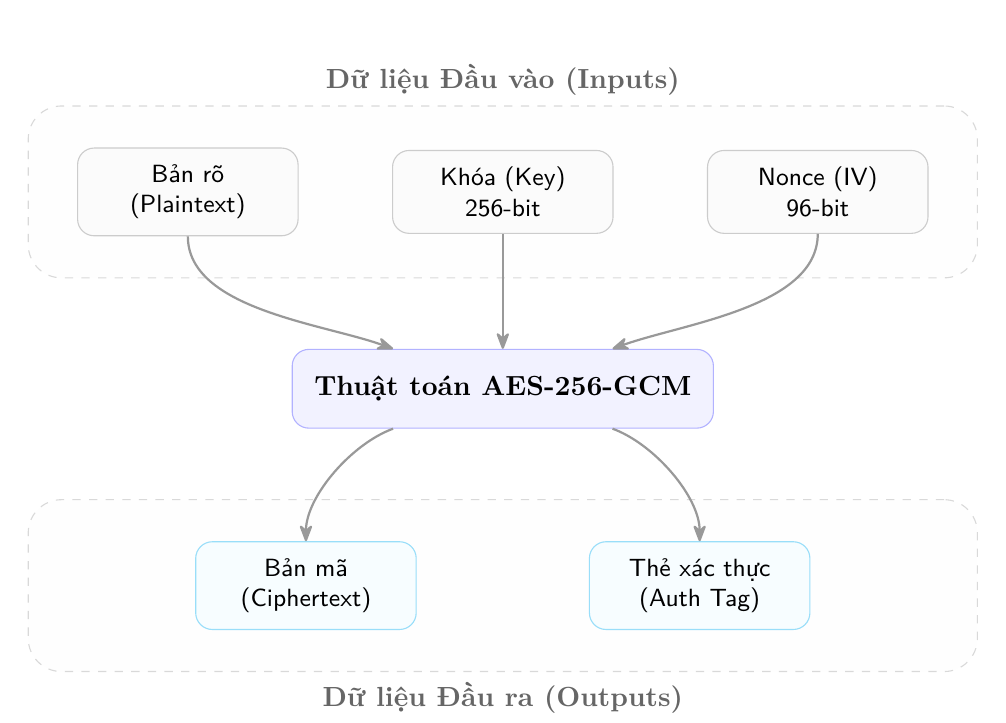
\begin{tikzpicture}[
    font=\sffamily\small,
    >={Stealth[round, scale=1.1]},
    box/.style={draw=blue!30, fill=blue!5, rounded corners=6pt, inner sep=8pt, align=center, minimum height=1cm, minimum width=3.5cm, font=\bfseries},
    input/.style={draw=gray!40, fill=gray!3, rounded corners=6pt, inner sep=6pt, align=center, minimum height=0.9cm, minimum width=2.8cm},
    output/.style={draw=cyan!40, fill=cyan!3, rounded corners=6pt, inner sep=6pt, align=center, minimum height=0.9cm, minimum width=2.8cm},
    arrow/.style={->, thick, gray!80, rounded corners=4pt},
    region/.style={draw=gray!30, dashed, rounded corners=12pt, inner sep=15pt, fill=gray!1}
]

% PROCESSING
\node[box] (aes) at (0,0) {Thuật toán AES-256-GCM};

% INPUTS
\node[input] (key) at (0, 2.5) {Khóa (Key)\\256-bit};
\node[input] (plain) at (-4, 2.5) {Bản rõ\\(Plaintext)};
\node[input] (iv) at (4, 2.5) {Nonce (IV)\\96-bit};

% OUTPUTS
\node[output] (cipher) at (-2.5, -2.5) {Bản mã\\(Ciphertext)};
\node[output] (tag) at (2.5, -2.5) {Thẻ xác thực\\(Auth Tag)};

% ARROWS - INPUTS to AES
\draw[arrow, out=-90, in=160, looseness=0.8] (plain.south) to (aes.160);
\draw[arrow] (key.south) -- (aes.north);
\draw[arrow, out=-90, in=20, looseness=0.8] (iv.south) to (aes.20);

% ARROWS - AES to OUTPUTS
\draw[arrow, out=200, in=90, looseness=0.8] (aes.200) to (cipher.north);
\draw[arrow, out=-20, in=90, looseness=0.8] (aes.-20) to (tag.north);

% REGIONS
\begin{scope}[on background layer]
    \coordinate (pad_in_l) at (-5.5, 2.5);
    \coordinate (pad_in_r) at (5.5, 2.5);
    \node[region, fit=(plain) (key) (iv) (pad_in_l) (pad_in_r)] (reg_in) {};
    \node[anchor=south, font=\bfseries\color{gray!80!black}] at (reg_in.north) {Dữ liệu Đầu vào (Inputs)};
    
    \coordinate (pad_out_l) at (-5.5, -2.5);
    \coordinate (pad_out_r) at (5.5, -2.5);
    \node[region, fit=(cipher) (tag) (pad_out_l) (pad_out_r)] (reg_out) {};
    \node[anchor=north, font=\bfseries\color{gray!80!black}] at (reg_out.south) {Dữ liệu Đầu ra (Outputs)};
\end{scope}

\end{tikzpicture}
\caption{Mô hình tổng quan đầu vào và đầu ra của thuật toán AES-GCM}
\label{fig:aes_gcm}
\end{figure}

\subsection{Lý do chọn AES-256-GCM}
Quyết định neo chặt kiến trúc vào AES-256-GCM xuất phát từ bốn trụ cột kỹ thuật mang tính thực tiễn cao:
\begin{enumerate}
    \item \textbf{Kháng cự lại sự ngụy tạo (Tamper Resistance):} Trong môi trường mạng phi tín nhiệm, thao túng bản mã (ciphertext malleability attack) là một chiến thuật nhắm thẳng vào tính toàn vẹn của dữ liệu. Kẻ thù có thể chặn bắt và sửa đổi vài bit ngẫu nhiên của gói tin. Khác với CBC, cơ chế Authentication Tag của GCM đóng vai trò như một người gác cổng. Hàm giải mã sẽ vứt bỏ thẳng thừng bất kỳ khối dữ liệu nào không khớp mã xác thực, hạn chế tối đa rủi ro hệ thống bị lợi dụng làm \textit{Oracle} để dò đoán bản rõ.
    \item \textbf{Tăng tốc bằng phần cứng (Hardware Acceleration):} Nhược điểm cố hữu của mã hóa Client-side là sự phụ thuộc nặng nề vào năng lực tính toán của máy khách. Dù vậy, AES-GCM được ưu ái bởi hầu hết các vi xử lý (CPU) hiện đại. Nhờ tích hợp sẵn tập lệnh chuyên biệt (chẳng hạn AES-NI) để giải quyết phép toán Galois, sự đánh đổi (trade-off) giữa bảo mật và hiệu năng được dung hòa xuất sắc, ép độ trễ mã hóa xuống mức mili-giây.
    \item \textbf{Khử rủi ro chuỗi cung ứng (Supply Chain Security):} Thay vì nhập nhằng với hàng loạt thư viện mã nguồn mở tiềm ẩn lỗ hổng (như các gói NPM), AES-GCM được trình duyệt thực thi trực tiếp qua \textit{Web Cryptography API} (\textcite{w3c-webcrypto-2017}). Việc vận hành nguyên bản (native) ở mức hệ điều hành giúp thu hẹp đáng kể bề mặt tấn công. 
    \item \textbf{Phòng ngự chiều sâu trước Điện toán lượng tử (Post-Quantum Defense):} Dưới sự đe dọa của thuật toán Grover trên máy tính lượng tử, sức mạnh của một hệ mật đối xứng sẽ bị suy giảm theo hàm căn bậc hai \parencite{nist-ir8105-pqc}. Nghĩa là một khóa 256-bit sẽ bị ép xuống mức độ khó tương đương khóa 128-bit. Mặc dù vậy, mốc 128-bit lượng tử vẫn là một bức tường thành vật lý quá sức đối với các siêu máy tính trong nhiều thập kỷ tới. Lựa chọn này giúp Secret Letter duy trì sự miễn nhiễm lâu dài trước những bước tiến của khoa học mật mã tương lai.
\end{enumerate}

Việc nhúng AES-256-GCM vào lõi hệ thống cung cấp một lời giải vẹn toàn: vừa gia tăng đáng kể độ khó cho tin tặc thông qua không gian khóa khổng lồ, vừa bảo vệ tính nguyên vẹn của luồng giao tiếp mà không vắt kiệt tài nguyên thiết bị của người dùng cuối.
\section{Kiến trúc Client-Side Encryption}

\subsection{Khái niệm và Nguyên lý hoạt động}
Mã hóa phía máy khách (Client-Side Encryption - CSE) là một mô hình bảo mật mà trong đó, quá trình mã hóa dữ liệu được thực hiện hoàn toàn trên thiết bị của người dùng (như trình duyệt web, điện thoại di động) trước khi bất kỳ dữ liệu nào được truyền tải qua mạng lưới internet hoặc lưu trữ trên máy chủ của bên thứ ba. 

Trái ngược với mã hóa phía máy chủ (Server-Side Encryption) – nơi máy chủ nắm giữ cả bản rõ và khóa giải mã – kiến trúc CSE đảm bảo rằng máy chủ trung gian đóng vai trò như một hệ thống "mù" (Zero-Knowledge). Máy chủ chỉ lưu trữ các cụm dữ liệu đã được mã hóa ngẫu nhiên và hoàn toàn không có khả năng đọc, phân tích hay khôi phục lại nội dung gốc do không sở hữu khóa bí mật.

\subsection{Sơ đồ kiến trúc toàn trình (End-to-End)}
Để hiện thực hóa mô hình Zero-Knowledge trong dự án \textit{Secret Letter}, kiến trúc truyền tải dữ liệu và khóa giải mã được thiết kế như sơ đồ Hình \ref{fig:cse_arch} dưới đây:

\begin{figure}[H]
\centering
\resizebox{\textwidth}{!}{
\input{img/cse_architecture.tex}
}
\caption{Kiến trúc Client-Side Encryption và cơ chế phân phối khóa qua URL Fragment}
\label{fig:cse_arch}
\end{figure}

\subsection{Cơ chế bảo vệ bằng URL Fragment}
Một trong những thách thức lớn nhất của Client-Side Encryption là làm thế nào để truyền tải khóa giải mã từ người gửi đến người nhận một cách an toàn mà không bị máy chủ trung gian đánh chặn. \textit{Secret Letter} giải quyết triệt để vấn đề này bằng cách tận dụng thuộc tính \textbf{URL Fragment} (phần chuỗi ký tự đứng sau dấu thăng \texttt{\#}).

Theo đặc tả giao thức HTTP do W3C và IETF quy định, các trình duyệt web khi thực hiện các truy vấn GET đến một máy chủ sẽ \textbf{tuyệt đối không bao giờ gửi phần Fragment} trong HTTP Request. Đoạn văn bản sau dấu \texttt{\#} chỉ tồn tại ở bộ nhớ cục bộ (local memory) của trình duyệt để xử lý logic nội bộ.

Trong dự án:
\begin{enumerate}
    \item \textbf{Phía gửi:} Khóa AES-256-GCM ngẫu nhiên được mã hóa dạng \texttt{Base64Url} và đính kèm vào đường dẫn (ví dụ: \texttt{https://secret.quorix.io.vn/secret/12345\#Kh0aB1M4t}). Phần bản mã được gửi lên máy chủ lưu trữ với định danh là \texttt{12345}.
    \item \textbf{Phía nhận:} Khi người dùng truy cập vào liên kết, trình duyệt gửi yêu cầu lấy bản mã dựa vào ID \texttt{12345}. Sau khi nhận được bản mã từ máy chủ, mã JavaScript trên trình duyệt của người nhận sẽ trích xuất khóa \texttt{Kh0aB1M4t} từ thanh địa chỉ để tiến hành giải mã cục bộ.
\end{enumerate}

Cơ chế này mang lại độ bảo mật vượt trội: ngay cả khi máy chủ Backend bị tin tặc chiếm quyền điều khiển hoàn toàn và thu thập toàn bộ cơ sở dữ liệu, chúng cũng chỉ có trong tay những chuỗi ký tự vô nghĩa vì \textbf{khóa giải mã chưa bao giờ rời khỏi thiết bị của người dùng để đi lên mạng Internet}. Điều này thiết lập nên kiến trúc Zero-Knowledge đúng nghĩa.
\section{Công nghệ Backend}

Kiến trúc Backend của \textit{Secret Letter} được thiết kế với mục tiêu tối giản, an toàn và tối ưu hóa hiệu suất xử lý luồng. Hệ thống từ bỏ các framework cồng kềnh để tập trung vào một tập lệnh biên dịch duy nhất, kết hợp với cơ sở dữ liệu xử lý trên bộ nhớ (in-memory) nhằm đáp ứng yêu cầu độ trễ thấp.

\subsection{Ngôn ngữ lập trình Go}
Ngôn ngữ Go (Golang) được lựa chọn làm nền tảng phát triển dịch vụ máy chủ nhờ đặc tính biên dịch tĩnh và khả năng quản lý đồng thời (concurrency) xuất sắc. 

Khác với các ngôn ngữ thông dịch đòi hỏi môi trường thực thi phức tạp, Go cho phép đóng gói toàn bộ mã nguồn và thư viện phụ thuộc vào một tệp thực thi duy nhất (single binary). Quyết định kỹ thuật này không chỉ tinh gọn quá trình triển khai mà còn thu hẹp đáng kể bề mặt tấn công sinh ra từ các lỗi chuỗi cung ứng (supply chain vulnerabilities). Bên cạnh đó, việc khai thác trực tiếp thư viện chuẩn \texttt{net/http} giúp hệ thống duy trì khả năng tiếp nhận và xử lý hàng nghìn kết nối đồng thời mà không bị kìm hãm bởi chi phí phân bổ bộ nhớ (memory allocation overhead) của các middleware dư thừa.

\subsection{Lưu trữ và Thao tác nguyên tử với Redis}
Tính năng cốt lõi của hệ thống là đảm bảo một thông điệp chỉ được phép hiển thị đúng một lần duy nhất (read-once). Đặc tả này đặt ra một bài toán kỹ thuật lớn về tương tranh (race condition): nếu kẻ tấn công gửi cùng lúc nhiều yêu cầu truy xuất cho một mã định danh, máy chủ có thể vô tình phản hồi bản mã cho nhiều hơn một đối tượng trước khi tiến trình xóa kịp thực thi.

Để giải quyết rủi ro này, hệ thống tích hợp Redis làm cơ sở dữ liệu chính và áp dụng kỹ thuật thao tác nguyên tử thông qua \textbf{Lua Script}. Thay vì tách rời các lệnh đọc và xóa, kịch bản Lua (như \texttt{claimOpenSecretScript}) gộp nhóm toàn bộ thao tác thành một khối thống nhất. Khi chuỗi lệnh này được đưa vào bộ máy thực thi luồng đơn (single-threaded) của Redis, không có bất kỳ lệnh nào khác được phép xen ngang. Nhờ vậy, ngay cả trong kịch bản hàng trăm yêu cầu ập đến cùng lúc, chỉ có yêu cầu đầu tiên trích xuất thành công, trong khi phần còn lại sẽ lập tức bị từ chối do trạng thái thông điệp đã thay đổi.

\subsection{Cơ chế bảo vệ biên và Mã hóa tại chỗ (At-Rest Encryption)}
Mặc dù dữ liệu đã được áp dụng Client-Side Encryption trước khi rời khỏi thiết bị người dùng, Backend vẫn thiết lập một loạt cơ chế kiểm soát nhằm bảo vệ tài nguyên máy chủ trước các luồng giao thông bất thường.

\begin{itemize}
    \item \textbf{Mã hóa tại chỗ (At-Rest):} Dù bản mã nhận được từ máy khách vốn đã không thể đọc lén, hệ thống tiếp tục áp dụng thêm một lớp mã hóa máy chủ bằng thuật toán AES-256-GCM trước khi ghi vào bộ nhớ Redis. Khóa nội bộ này được quản lý độc lập thông qua biến môi trường. Lớp bảo vệ này đóng vai trò giới hạn phạm vi rò rỉ trong trường hợp bản thân dịch vụ Redis bị xâm nhập trái phép.
    \item \textbf{Giới hạn tải trọng (Payload Restriction):} Dung lượng của mọi yêu cầu HTTP gửi đến bộ xử lý bị ràng buộc chặt chẽ ở mức tối đa 15KB bằng hàm \texttt{http.MaxBytesReader}. Cơ chế này nhằm chủ động giảm thiểu rủi ro cạn kiệt bộ nhớ máy chủ (OOM) hoặc tấn công làm ngập lụt tài nguyên thông qua việc bơm dữ liệu kích thước lớn.
    \item \textbf{Kiểm soát lưu lượng (Rate Limiting):} Hệ thống duy trì một bộ định mức luồng (rate limiter) vận hành trực tiếp trên Redis. Bằng cách trích xuất an toàn địa chỉ IP thực của thiết bị đầu cuối qua tiêu đề \texttt{X-Forwarded\--For} từ các dải proxy được ủy thác, máy chủ thiết lập hạn mức kết nối riêng biệt cho từng loại giao dịch (tạo mới, truy xuất, kiểm tra trạng thái), từ đó hạn chế đáng kể khả năng dò quét (brute-force) mã thông điệp.
\end{itemize}
\section{Công nghệ Frontend}

Giao diện người dùng của \textit{Secret Letter} được xây dựng dựa trên các công nghệ web hiện đại, ưu tiên tốc độ phản hồi và tính bảo mật cao khi thao tác với dữ liệu nhạy cảm.

\subsection{Thư viện React và Công cụ biên dịch Vite}
Hệ thống sử dụng thư viện React làm cốt lõi để kiến tạo giao diện Frontend. Điểm mạnh của React nằm ở kiến trúc Component, cho phép phân rã các khu vực chức năng (như biểu mẫu nhập liệu, hộp thoại hiển thị khóa, màn hình kết quả) thành các thành phần độc lập và có khả năng tái sử dụng. Cơ chế quản lý trạng thái (state management) nội tại giúp giao diện phản hồi tức thời với các tương tác của người dùng mà không đòi hỏi thao tác tải lại trang (page reload).

Song song đó, dự án tích hợp Vite làm công cụ biên dịch (build tool) chính. Bằng cách khai thác cơ chế ES Modules tiêu chuẩn của trình duyệt, Vite tăng tốc đáng kể quá trình phát triển thông qua tính năng Hot Module Replacement (HMR). Ở môi trường thực tế (production), mã nguồn được Vite đóng gói thành các tệp tĩnh (static assets) với kích thước tối ưu, giúp giảm thiểu độ trễ tải trang ngay cả khi người dùng truy cập từ các mạng băng thông thấp.

\subsection{Xử lý Mật mã với Web Cryptography API}
Theo kiến trúc mã hóa máy khách (Client-Side Encryption), toàn bộ quy trình biến đổi bản rõ thành bản mã phải được hoàn tất trên trình duyệt. Nếu phụ thuộc vào các thư viện mật mã viết thuần bằng JavaScript (chẳng hạn như CryptoJS), hệ thống sẽ đối mặt với sự suy giảm hiệu năng kết xuất và tiềm ẩn rủi ro bảo mật từ các chuỗi cung ứng (supply chain attack) do sử dụng gói phần mềm bên thứ ba.

Để giải quyết bài toán này, hệ thống giao phó hoàn toàn trách nhiệm tính toán cho \textbf{Web Cryptography API} (\textcite{w3c-webcrypto-2017}). Đây là một tiêu chuẩn của W3C được tích hợp sâu vào bộ lõi của mọi trình duyệt web hiện đại. Việc gọi hàm mã hóa thuật toán AES-GCM qua API này cung cấp đặc quyền truy cập trực tiếp vào các tập lệnh mật mã cấp thấp (low-level) do hệ điều hành quản lý. Thiết kế này không chỉ gia tăng tốc độ mã hóa thông qua khả năng tăng tốc phần cứng, mà còn giới hạn rủi ro lộ lọt bộ nhớ so với việc duy trì dữ liệu khóa trực tiếp trong không gian JavaScript.

\subsection{Thiết kế UI/UX và Trải nghiệm điện ảnh (Cinematic Experience)}
Khác với các ứng dụng tiện ích thông thường, \textit{Secret Letter} hướng tới một trải nghiệm thị giác mang tính điện ảnh (Dark Cinematic). Hệ thống chủ động từ bỏ các bộ khung CSS cồng kềnh để làm chủ hoàn toàn giao diện thông qua \textbf{Vanilla CSS} và CSS Variables. Quyết định này giúp kiến tạo một bảng màu phối hợp (color scheme) đặc trưng như xanh đen sâu, vàng kim và phông chữ cổ điển có chân (\textit{Playfair Display}), mô phỏng lại cảm giác đọc một bức thư bí mật chân thực.

Điểm nhấn kỹ thuật nằm ở việc ứng dụng thư viện \textbf{GSAP} (GreenSock Animation Platform) để điều hướng các chuyển động. Thay vì phụ thuộc vào các hiệu ứng chuyển tiếp (transition) đơn giản của CSS dễ gây suy giảm khung hình trên thiết bị cấu hình thấp, GSAP cho phép đồng bộ hóa các mốc thời gian (timelines) phức tạp ở hiệu năng cao. Cơ chế này mang lại các hiệu ứng mở thư và xuất hiện mượt mà, củng cố tính nhập vai (immersive) của người dùng đồng thời hạn chế tối đa chi phí tiêu hao tài nguyên kết xuất (rendering overhead).
\chapter{PHÂN TÍCH VÀ THIẾT KẾ HỆ THỐNG}
\section{Phân tích yêu cầu}

Tài liệu đặc tả (Product Specification) của \textit{Secret Letter} phân hoạch hệ thống thành ba nhóm yêu cầu cốt lõi, đặt trọng tâm vào việc giải quyết bài toán chia sẻ thông tin nhạy cảm một lần duy nhất mà không đòi hỏi sự tin tưởng vào máy chủ lưu trữ (Zero-Trust Model).

\subsection{Yêu cầu chức năng (Functional Requirements)}
Hệ thống xoay quanh một vòng đời dữ liệu khép kín, được định hình bởi các nghiệp vụ chính:

\begin{itemize}
    \item \textbf{Mã hóa và Tạo liên kết (FR-1 \& FR-2):} Người gửi soạn thảo văn bản (tối đa 10KB). Trình duyệt tiến hành mã hóa bằng Web Crypto API (AES-256-GCM) trước khi truyền tải, trả về liên kết chia sẻ dạng \texttt{URL\#FragmentKey}.
    \item \textbf{Phòng vệ trước Bot tự động (FR-3 - Preview Bot Protection):} Để tránh việc các Bot xem trước (như Crawler của Zalo, Telegram) vô tình tiêu thụ thông điệp, trình duyệt không tự động giải mã khi tải trang. Việc giải mã yêu cầu tương tác chủ đích (click chuột) từ người dùng.
    \item \textbf{Tiêu thụ Nguyên tử (FR-4 - Atomic Consumption):} Cơ chế đảm bảo thông điệp chỉ được trích xuất thành công một lần. Các yêu cầu truy xuất tiếp theo sẽ bị từ chối.
    \item \textbf{Vòng đời tự động (FR-5 - TTL-Based Expiration):} Hệ thống hỗ trợ cơ chế dọn dẹp theo thời gian (1 giờ, 24 giờ, 7 ngày) qua hàm EXPIRE của Redis.
    \item \textbf{Trạng thái minh bạch (FR-6) và Giới hạn (FR-7):} Người nhận được thông báo rõ ràng về tình trạng của liên kết (\textit{Đã bị tiêu thụ}, \textit{Đã hết hạn}). Hệ thống áp dụng hạn mức kết nối (ví dụ: 120 yêu cầu tạo/giờ/IP) nhằm giảm thiểu lạm dụng.
\end{itemize}

Dưới đây là sơ đồ luồng người dùng thể hiện rõ chốt chặn "Tương tác chủ đích" để phòng chống Bot:

\begin{figure}[H]
\centering
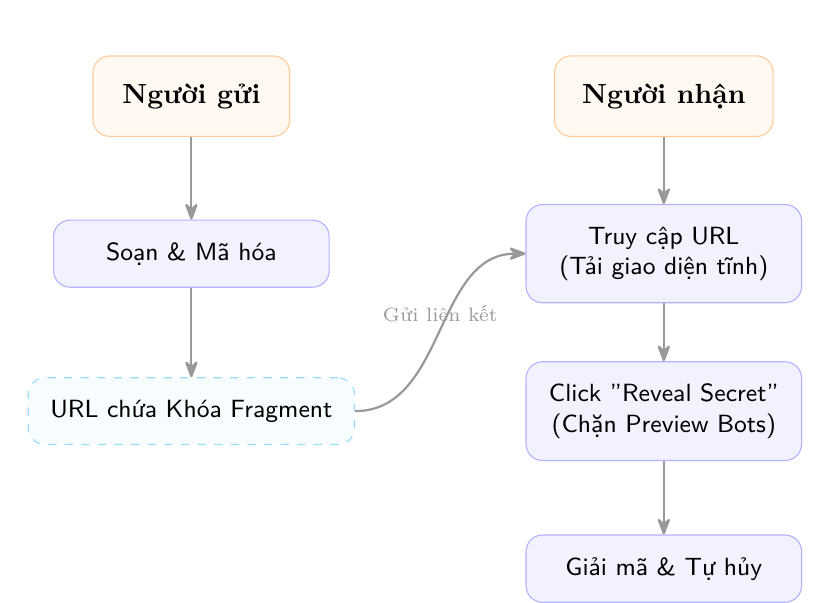
\begin{tikzpicture}[
    font=\sffamily\small,
    >={Stealth[round, scale=1.1]},
    actor/.style={draw=orange!40, fill=orange!5, rounded corners=6pt, inner sep=10pt, align=center, font=\bfseries, minimum width=2.5cm},
    action/.style={draw=blue!30, fill=blue!5, rounded corners=6pt, inner sep=8pt, align=center, minimum height=0.8cm, minimum width=3.5cm},
    data/.style={draw=cyan!40, fill=cyan!3, rounded corners=6pt, inner sep=8pt, align=center, minimum height=0.8cm, minimum width=3.5cm, dashed},
    arrow/.style={->, thick, gray!80, rounded corners=4pt}
]

% Nodes
\node[actor] (sender) at (0, 6) {Người gửi};
\node[action] (create) at (0, 4) {Soạn \& Mã hóa};
\node[data] (link) at (0, 2) {URL chứa Khóa Fragment};

\node[actor] (receiver) at (6, 6) {Người nhận};
\node[action] (access) at (6, 4) {Truy cập URL\\(Tải giao diện tĩnh)};
\node[action] (click) at (6, 2) {Click "Reveal Secret"\\(Chặn Preview Bots)};
\node[action] (read) at (6, 0) {Giải mã \& Tự hủy};

% Arrows
\draw[arrow] (sender) -- (create);
\draw[arrow] (create) -- (link);
\draw[arrow, out=0, in=180] (link.east) to node[midway, above, font=\scriptsize\color{gray!80!black}] {Gửi liên kết} (access.west);
\draw[arrow] (receiver) -- (access);
\draw[arrow] (access) -- (click);
\draw[arrow] (click) -- (read);

\end{tikzpicture}
\caption{Luồng tương tác cốt lõi của người dùng tích hợp cơ chế chống Bot (User Flow)}
\label{fig:req_user_flow}
\end{figure}

\subsection{Yêu cầu an toàn thông tin (Security Requirements)}
Dự án duy trì các đường cơ sở bảo mật nghiêm ngặt xuyên suốt các thành phần:
\begin{itemize}
    \item \textbf{Lưu trữ và Truyền tải (SR-1 \& SR-4):} Hệ thống được thiết kế để máy chủ không lưu giữ khóa giải mã. Toàn bộ giao tiếp thực hiện qua HTTPS kèm theo các tiêu đề HSTS, CSP. Bản mã được bảo vệ thêm một lớp (At-Rest) tại cơ sở dữ liệu.
    \item \textbf{Kiểm soát dữ liệu đầu vào (SR-5):} Dữ liệu từ Client bị giới hạn (tối đa 15KB). Các thao tác kết nối và xử lý trên Redis được thiết lập thời gian chờ khắt khe (ở mức hàng chục mili-giây) nhằm hạn chế rủi ro treo tiến trình khi hệ thống chịu tải cao.
\end{itemize}

\subsection{Yêu cầu phi chức năng (Non-Functional Requirements)}
Nhằm đảm bảo dự án có khả năng duy trì, vận hành và nâng cấp trong tương lai, hệ thống tuân thủ 4 tiêu chuẩn cốt lõi:
\begin{itemize}
    \item \textbf{Độ trễ (NFR-1 - Latency):} Các giao diện lập trình ứng dụng (API) tạo và truy xuất được thiết kế để phản hồi ở mức tối ưu. Thao tác mã hóa và giải mã cần hoạt động hiệu quả trên đa số các thiết bị di động.
    \item \textbf{Độ tin cậy (NFR-2 - Reliability):} Cơ chế tự hủy (reveal) cần duy trì tính chính xác (đúng một lần) dưới áp lực truy cập đồng thời. Việc khởi động lại dịch vụ không làm ảnh hưởng các liên kết đang hiệu lực.
    \item \textbf{Tính tối giản (NFR-3 - Simplicity):} Phiên bản MVP thiết kế gọn nhẹ để có thể chạy cục bộ với tổ hợp \texttt{Frontend + Go Services + Redis}. Mỗi dịch vụ đảm nhiệm một trách nhiệm cụ thể.
    \item \textbf{Khả năng vận hành (NFR-4 - Operability):} Môi trường phát triển cục bộ hoạt động trơn tru qua \texttt{Docker Compose}. Khi triển khai, kiến trúc hỗ trợ khả năng mở rộng ngang (horizontal scaling) đối với các dịch vụ phi trạng thái.
\end{itemize}
\section{Kiến trúc tổng thể}

Kiến trúc của hệ thống \textit{Secret Letter} được thiết kế theo mô hình Nguyên khối Mô-đun hóa (Modular Monolith) ở giai đoạn MVP. Lựa chọn này bắt nguồn từ nhu cầu tối ưu hóa chi phí vận hành ban đầu, đồng thời vẫn phải duy trì tính kỷ luật trong việc phân định ranh giới dịch vụ (Service Boundaries). Sự tách bạch logic nội bộ ngay từ sớm tạo tiền đề để hệ thống có thể chuyển đổi mượt mà sang kiến trúc vi dịch vụ (Microservices) khi quy mô dự án và lưu lượng truy cập mở rộng.

Căn cứ theo hướng dẫn của mô hình C4 (C4 Model) - Cấp độ 2 (Container Diagram), hệ sinh thái kỹ thuật của dự án được biểu diễn trực quan như sau:

\begin{figure}[H]
\centering
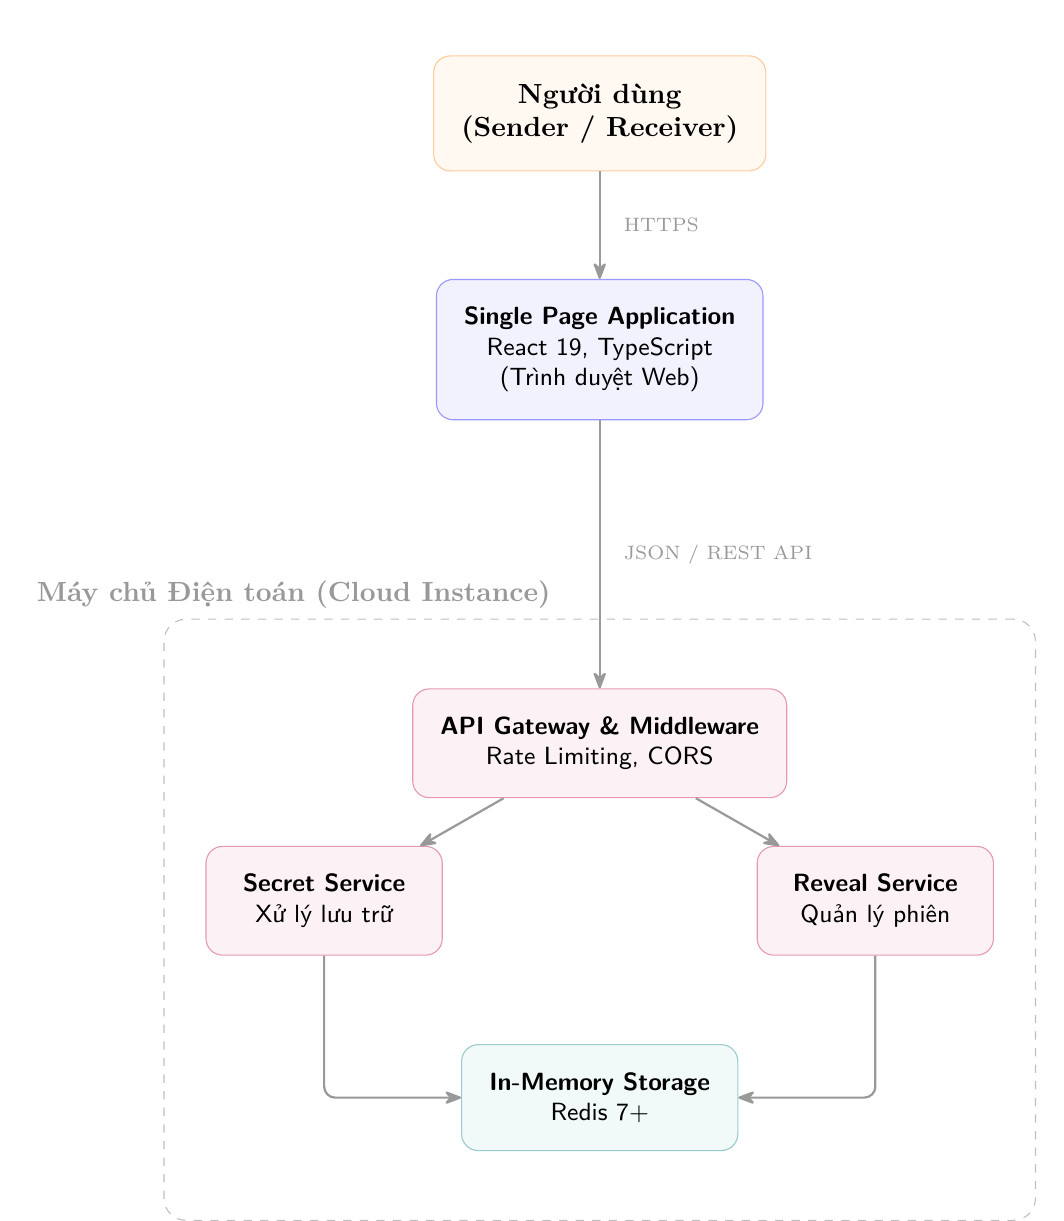
\begin{tikzpicture}[
    font=\sffamily\small,
    >={Stealth[round, scale=1.1]},
    user/.style={draw=orange!40, fill=orange!5, rounded corners=6pt, inner sep=10pt, align=center, font=\bfseries, minimum width=2.5cm},
    spa/.style={draw=blue!40, fill=blue!5, rounded corners=6pt, inner sep=10pt, align=center, minimum width=3cm, minimum height=1.2cm},
    api/.style={draw=purple!40, fill=purple!5, rounded corners=6pt, inner sep=10pt, align=center, minimum width=3cm, minimum height=1.2cm},
    db/.style={draw=teal!40, fill=teal!5, rounded corners=6pt, inner sep=10pt, align=center, minimum width=3cm, minimum height=1.2cm},
    group/.style={draw=gray!50, dashed, rounded corners=8pt, inner sep=15pt, inner ysep=25pt},
    arrow/.style={->, thick, gray!80, rounded corners=4pt}
]

% Nodes
\node[user] (user) at (0, 8) {Người dùng\\(Sender / Receiver)};

\node[spa] (frontend) at (0, 5) {\textbf{Single Page Application}\\React 19, TypeScript\\(Trình duyệt Web)};

% Backend Group
\node[api] (gateway) at (0, 0) {\textbf{API Gateway \& Middleware}\\Rate Limiting, CORS};
\node[api] (secretsvc) at (-3.5, -2) {\textbf{Secret Service}\\Xử lý lưu trữ};
\node[api] (revealsvc) at (3.5, -2) {\textbf{Reveal Service}\\Quản lý phiên};
\node[db] (redis) at (0, -4.5) {\textbf{In-Memory Storage}\\Redis 7+};

% Group boxes - Đặt label lệch trái (anchor=south east) để không đè lên mũi tên chính giữa
\node[group, fit=(gateway) (secretsvc) (revealsvc) (redis), label={[font=\bfseries, text=gray!80, anchor=south east, xshift=-0.5cm]above:Máy chủ Điện toán (Cloud Instance)}] (backend_group) {};

% Arrows - Đẩy text lệch phải (xshift=5pt) để nhường không gian cho mũi tên
\draw[arrow] (user) -- node[right, font=\scriptsize, align=left, xshift=5pt] {HTTPS} (frontend);
\draw[arrow] (frontend) -- node[right, font=\scriptsize, align=left, xshift=5pt] {JSON / REST API} (gateway);
\draw[arrow] (gateway) -- (secretsvc);
\draw[arrow] (gateway) -- (revealsvc);
\draw[arrow] (secretsvc) |- (redis);
\draw[arrow] (revealsvc) |- (redis);

\end{tikzpicture}
\caption{Sơ đồ Container (C4 Model - Mức 2) phân tách ranh giới dịch vụ}
\label{fig:c4_container}
\end{figure}

\subsection{Chi tiết các thành phần (Containers)}

Hệ thống được cấu thành từ ba khối thực thể độc lập, phối hợp với nhau qua các giao thức mạng chuẩn nhằm duy trì vòng đời thông điệp:

\begin{itemize}
    \item \textbf{Single Page Application (SPA):} Chịu trách nhiệm thực thi giao diện người dùng và logic mật mã học. Bằng việc tích hợp Web Crypto API, quá trình mã hóa/giải mã (AES-GCM) được thực thi trực tiếp tại máy khách. Điều này phản ánh nguyên lý Zero-Knowledge cốt lõi: hạn chế tối đa rủi ro văn bản rõ (plaintext) bị truyền tải vào đường mạng.
    
    \item \textbf{Máy chủ Ứng dụng (Backend Monolith):} Một tệp thực thi duy nhất (Single Binary) được biên dịch từ ngôn ngữ Go, tối ưu cho tốc độ và khả năng xử lý đồng thời. Dù chỉ là một tệp nhị phân, kiến trúc bên trong được chia cắt chặt chẽ theo miền nghiệp vụ:
    \begin{itemize}
        \item \textit{Lớp Gateway \& Middleware:} Đóng vai trò kiểm duyệt biên. Tầng này gán định danh (Request ID) cho mục đích truy vết, thiết lập chính sách CORS và thực thi cơ chế giới hạn lưu lượng (Rate Limiting) theo địa chỉ IP nhằm giảm thiểu tác động từ các đợt tấn công cạn kiệt tài nguyên.
        \item \textit{Secret Service:} Đảm nhận nghiệp vụ lưu trữ thông điệp mã hóa. Dịch vụ này giao tiếp với cơ sở dữ liệu để quản lý siêu dữ liệu (Metadata) và gán vòng đời (TTL).
        \item \textit{Reveal Service:} Chịu trách nhiệm cấp phát các phiên giải mã ngắn hạn (Reveal Session). Dịch vụ này thực thi kịch bản khóa nguyên tử nhằm hạn chế tối đa hiện tượng tương tranh (Race Condition) khi có nhiều yêu cầu mở liên kết cùng lúc.
    \end{itemize}
    
    \item \textbf{Cơ sở dữ liệu (In-Memory Storage):} Hệ quản trị Redis 7+ được thiết lập cục bộ. Điểm mạnh của Redis trong bài toán này nằm ở cấu trúc đơn luồng (Single-Threaded) kết hợp với Lua Script. Khả năng này cho phép hệ thống vận hành chuỗi lệnh "kiểm tra - trả về - xóa" một cách liền mạch, đảm bảo tính nguyên tử (atomic) của giao dịch.
\end{itemize}

\subsection{Chiến lược triển khai và Bảng phân tả công nghệ}

Triết lý triển khai của dự án hướng đến sự linh hoạt và tính sẵn sàng cao (High Availability). Các luồng giao tiếp chính được thiết lập qua một lớp Reverse Proxy chuyên dụng nhằm tự động hóa quá trình cấp phát chứng chỉ SSL/TLS và thiết lập mã hóa toàn trình. Song song với máy chủ điện toán chính yếu, một môi trường dự phòng (Warm Standby) liên tục được duy trì. Trong trường hợp phát sinh sự cố tại trung tâm dữ liệu chính, quản trị viên có thể thao tác điều hướng bản ghi DNS để phục hồi dịch vụ.

Dưới đây là bảng phân tả chi tiết bộ công nghệ (Tech Stack) áp dụng cho từng Container:

\begin{table}[H]
\centering
\caption{Bảng phân tả công nghệ theo Container}
\renewcommand{\arraystretch}{1.5}
\begin{tabular}{|p{3.5cm}|p{5cm}|p{6cm}|}
\hline
\textbf{Thành phần} & \textbf{Công nghệ cốt lõi} & \textbf{Lý do lựa chọn} \\
\hline
\textbf{Frontend (SPA)} & React 19, TypeScript, Web Crypto API, Vite & Hệ sinh thái mạnh mẽ, kiểm soát kiểu tĩnh chặt chẽ, tối ưu thuật toán mật mã học an toàn ngay trên trình duyệt. \\
\hline
\textbf{Backend (Monolith)} & Go 1.26+, \texttt{net/http} & Hiệu suất xử lý I/O mạng ưu việt (Goroutines), triển khai tinh gọn thông qua định dạng tệp thực thi độc lập. \\
\hline
\textbf{Database} & Redis 7+ & Cung cấp độ trễ siêu thấp cho thao tác truy xuất, tích hợp sẵn tập lệnh Lua nguyên tử phục vụ nghiệp vụ tự hủy. \\
\hline
\textbf{Reverse Proxy} & Caddy Server & Cấu hình tối giản, thiết kế hướng bảo mật (memory-safe), cơ chế tự động gia hạn chứng chỉ HTTPS. \\
\hline
\end{tabular}
\label{tab:tech_stack}
\end{table}
\section{Thiết kế luồng dữ liệu}
\section{Thiết kế API}

Hệ thống giao diện lập trình ứng dụng (API) của \textit{Secret Letter} được thiết kế theo tiêu chuẩn RESTful, đảm nhiệm vai trò cầu nối duy nhất giữa máy khách (Frontend) và bộ xử lý lưu trữ (Backend). Khác với các kiến trúc CRUD thông thường, lớp API này chịu trách nhiệm hỗ trợ thực thi các chính sách bảo mật biên (Edge Security) và quản lý vòng đời tiêu thụ dữ liệu một lần (One-time Reveal).

\subsection{Cấu trúc Middleware và Kiểm duyệt biên}

Để thu hẹp các bề mặt tấn công từ lớp mạng, các luồng dữ liệu HTTP trước khi chạm đến các bộ xử lý logic (Handlers) được yêu cầu đi qua một chuỗi Middleware phòng thủ theo chiều sâu (Defense in Depth). Kiến trúc này được định nghĩa trực tiếp tại mã nguồn \texttt{internal/\-httpapi/\-server.go}:

\begin{figure}[H]
\centering
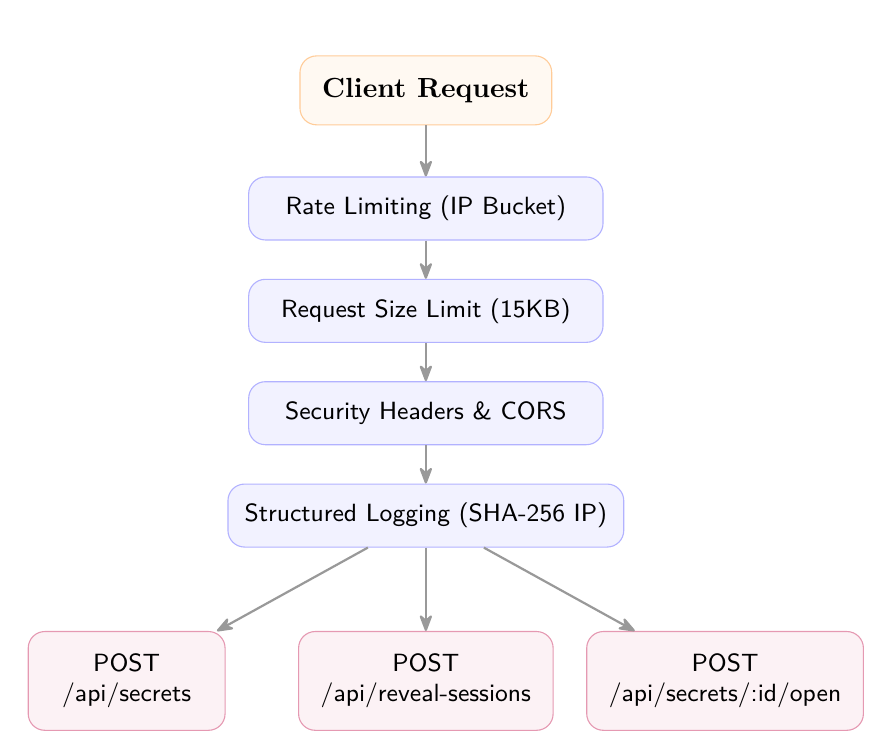
\begin{tikzpicture}[
    font=\sffamily\small,
    >={Stealth[round, scale=1.1]},
    client/.style={draw=orange!40, fill=orange!5, rounded corners=6pt, inner sep=8pt, align=center, font=\bfseries},
    middleware/.style={draw=blue!30, fill=blue!5, rounded corners=6pt, inner sep=6pt, align=center, minimum width=4.5cm, minimum height=0.8cm},
    handler/.style={draw=purple!40, fill=purple!5, rounded corners=6pt, inner sep=8pt, align=center, minimum width=2.5cm},
    arrow/.style={->, thick, gray!80, rounded corners=4pt}
]

\node[client] (client) at (0, 6) {Client Request};
\node[middleware] (mw1) at (0, 4.5) {Rate Limiting (IP Bucket)};
\node[middleware] (mw2) at (0, 3.2) {Request Size Limit (15KB)};
\node[middleware] (mw3) at (0, 1.9) {Security Headers \& CORS};
\node[middleware] (mw4) at (0, 0.6) {Structured Logging (SHA-256 IP)};

\node[handler] (h1) at (-3.8, -1.5) {POST\\/api/secrets};
\node[handler] (h2) at (0, -1.5) {POST\\/api/reveal-sessions};
\node[handler] (h3) at (3.8, -1.5) {POST\\/api/secrets/:id/open};

\draw[arrow] (client) -- (mw1);
\draw[arrow] (mw1) -- (mw2);
\draw[arrow] (mw2) -- (mw3);
\draw[arrow] (mw3) -- (mw4);
\draw[arrow] (mw4) -- (h1);
\draw[arrow] (mw4) -- (h2);
\draw[arrow] (mw4) -- (h3);

\end{tikzpicture}
\caption{Luồng xử lý yêu cầu đi qua hệ thống Middleware của API Gateway}
\label{fig:api_middleware_flow}
\end{figure}

Việc áp dụng các khối Middleware mang lại giá trị bảo mật hiện hữu:
\begin{itemize}
    \item \textbf{withRequestSizeLimit}: Hỗ trợ ngắt kết nối thông qua \texttt{http.\-MaxBytesReader} nếu tải trọng (Payload) vượt ngưỡng \texttt{15KB}, giúp ngăn chặn nguy cơ tấn công bơm rác làm tràn bộ nhớ (Data Flooding).
    \item \textbf{withSecurityHeaders}: Áp dụng các tiêu đề phản hồi bảo mật nhằm hạn chế rủi ro từ trình duyệt, bao gồm \texttt{Strict-Transport-Security (HSTS)} để yêu cầu dùng HTTPS, \texttt{X-Content-Type-Options: nosniff} chống đánh lừa định dạng, và \texttt{Content-Security-Policy (CSP)} nhằm kiểm soát nguồn thực thi mã.
    \item \textbf{withRequestLogging}: Bảo vệ quyền riêng tư bằng cách băm (hash) địa chỉ IP gốc và \texttt{User-Agent} bằng thuật toán SHA-256 trước khi xuất ra hệ thống Log nội bộ, đồng thời gắn kèm \texttt{X-Request-ID} dạng UUID để hỗ trợ truy vết.
\end{itemize}

\subsection{Đặc tả Endpoints cốt lõi}

Tài nguyên API được chia thành ba luồng thao tác bất biến, phản ánh vòng đời của một \textit{Secret}:

\subsubsection{Khởi tạo Thông điệp mã hóa}
Giao thức này tiếp nhận bản mã (ciphertext) đã được sinh ra tại trình duyệt và tiến hành lưu trữ vào In-Memory Database.
\begin{itemize}
    \item \textbf{Method \& Path:} \texttt{POST /api/secrets}
    \item \textbf{Headers bắt buộc:} \texttt{Content-Type: application/json}
    \item \textbf{Body Input:} Chứa các thuộc tính đã mã hóa bao gồm \texttt{ciphertext} (Bản mã Base64URL), \texttt{nonce} (IV khởi tạo ngẫu nhiên), \texttt{algorithm} (chuẩn thuật toán, mặc định là AES-GCM), và \texttt{ttlSeconds} (thời gian sống tính bằng giây).
    \item \textbf{Response Thành công (201 Created):} Trả về ID định danh nội bộ (\texttt{secretId}) và thời điểm sẽ bị tiêu hủy tự động (\texttt{expiresAt}).
    \item \textbf{Response Lỗi (4xx):} Trả về mã \texttt{413 Payload Too Large} nếu cấu trúc JSON vượt 15KB, hoặc mã \texttt{400 Validation Failed} nếu Request thiếu trường thông tin hợp lệ.
\end{itemize}

\subsubsection{Cơ chế Anti-Bot và Phiên giải mã (Reveal Session)}
Là cơ chế hỗ trợ ngăn ngừa các công cụ xem trước (Preview Bots) như Zalo, Telegram, Discord tự động tiêu thụ liên kết bí mật.
\begin{itemize}
    \item \textbf{Method \& Path:} \texttt{POST /api/reveal-sessions}
    \item \textbf{Vận hành:} Khi người nhận truy cập lần đầu tiên, giao diện sẽ gửi yêu cầu cấp một phiên làm việc (Session) ngắn hạn gắn với \texttt{secretId} đó. Thao tác này là bằng chứng xác thực có một người dùng thực sự đang chờ bấm nút "Mở thư".
    \item \textbf{Response (201 Created):} Cấp phát mã \texttt{sessionId} tạm thời để sử dụng cho bước tiếp theo.
\end{itemize}

\subsubsection{Truy vấn Trạng thái và Tiêu thụ (Consume)}
Hai API này đảm nhận khâu cuối cùng trong vòng đời thông điệp. Điểm đặc biệt của toàn bộ nhóm API \texttt{/secrets/:id/*} là máy chủ sẽ chủ động chèn thêm Header \texttt{Cache-Control: no-store} nhằm hạn chế tình trạng trình duyệt tải lại nội dung cũ đã bị xóa.
\begin{itemize}
    \item \textbf{\texttt{GET /api/secrets/:id/status}:} Trả về trạng thái hiện hành của thư (\texttt{active}, \texttt{consumed}, \texttt{expired}, \texttt{not\_found}) nhưng không thực thi việc xóa. Dùng để render giao diện kiểm tra.
    \item \textbf{\texttt{POST /api/secrets/:id/open} (hoặc \texttt{/consume}):} Kích hoạt chuỗi lệnh Lua Script nguyên tử trên Redis để trả về nguyên trạng bản mã, và ngay lập tức thực thi lệnh xóa sổ (DEL) bản ghi. Yêu cầu truyền vào Header \texttt{X-Reveal-Session} từ bước số 2 để chứng thực tính hợp lệ. Giao dịch thành công trả về \texttt{200 OK} kèm dữ liệu; nếu thất bại do thư đã bốc hơi, trả về \texttt{410 Gone} kèm thông báo chuẩn hóa.
\end{itemize}

\subsection{Vòng đời Thông điệp (Secret Lifecycle)}

Sự tương tác giữa các API nói trên cấu thành một vòng đời dữ liệu khép kín (như minh họa tại Hình \ref{fig:api_state_lifecycle}).

Việc định nghĩa rõ ràng các trạng thái (\texttt{active}, \texttt{consumed}, \texttt{expired}, \texttt{not\_found}) giúp hệ thống phản ứng linh hoạt trước các tình huống thực tế. Đặc biệt, thao tác tiêu hủy được thiết kế để thi hành ngay lập tức (Atomic DEL) khi người dùng mở thư, hoặc được hệ thống tự động dọn dẹp bởi cơ chế Key Eviction của Redis khi cạn thời gian sống (TTL). Điều này đóng vai trò quyết định trong việc duy trì nguyên lý "chỉ đọc một lần" (Burn-after-reading) của dự án.

\begin{figure}[H]
    \centering
    
\includegraphics[width=1.0\textwidth]{img/state_lifecycle.png}
    \caption{Sơ đồ trạng thái minh họa vòng đời lưu trữ của một thông điệp}
    \label{fig:api_state_lifecycle}
\end{figure}

\subsection{Tiêu chuẩn hóa Quản lý lỗi (Error Handling)}
Các phản hồi lỗi từ API được thiết kế để không trả về chuỗi văn bản thuần (raw string). Thay vào đó, bộ Middleware của Backend trừu tượng hóa các lỗi này thành cấu trúc \texttt{AppError} chuẩn hóa. Khối JSON lỗi mang định dạng \texttt{\{"code": "...", "message": "...", "details": \{...\}\}}. Cách tiếp cận này (nhất quán trong toàn bộ \texttt{handlers.go}) giúp quy trình xử lý trên Frontend trở nên thuận tiện hơn, hỗ trợ ánh xạ logic hiển thị lỗi (Error Boundary UI) một cách rõ ràng theo từng mã định danh cục bộ.
\chapter{TRIỂN KHAI CHI TIẾT}
\section{Cấu trúc mã nguồn}

Dự án \textit{Secret Letter} được tổ chức theo mô hình \textbf{Monorepo} (Lưu trữ đơn khối), nơi toàn bộ mã nguồn của Máy khách (Frontend), Máy chủ (Backend), tài liệu kỹ thuật và kịch bản triển khai được quy tụ trong một kho lưu trữ (Repository) duy nhất. 

Cách tiếp cận này mang lại lợi thế lớn trong việc duy trì tính đồng nhất (Consistency) giữa hợp đồng giao tiếp (API Contracts) và logic mật mã học. Bất kỳ thay đổi nào liên quan đến cấu trúc bản mã (Ciphertext) hay chuẩn mã hóa đều có thể được triển khai và kiểm thử đồng bộ trên cả hai nền tảng mà không gặp phải rào cản phân mảnh phiên bản (Version drift).

Dưới đây là sơ đồ biểu diễn các vùng kỹ thuật hạt nhân của dự án:

\vspace{0.5cm}
\begin{figure}[H]
    \centering
    \begin{minipage}{0.9\textwidth}
        \dirtree{%
        .1 \normalfont secret-letter/.
        .2 \normalfont backend/ \dots{} \begin{minipage}[t]{8cm}\normalfont Máy chủ Ứng dụng (Golang)\end{minipage}.
        .3 \normalfont cmd/api/ \dots{} \begin{minipage}[t]{8cm}\normalfont Điểm khởi chạy nhị phân (Entrypoint)\end{minipage}.
        .3 \normalfont internal/ \dots{} \begin{minipage}[t]{8cm}\normalfont Các mô-đun nghiệp vụ nội bộ\end{minipage}.
        .4 \normalfont httpapi/ \dots{} \begin{minipage}[t]{8cm}\normalfont Quản lý Middleware và REST Handlers\end{minipage}.
        .4 \normalfont secret/ \dots{} \begin{minipage}[t]{8cm}\normalfont Xác thực điều kiện và quản lý vòng đời\end{minipage}.
        .4 \normalfont store/ \dots{} \begin{minipage}[t]{8cm}\normalfont Giao tiếp Redis (thực thi Lua Scripts)\end{minipage}.
        .2 \normalfont deploy/ \dots{} \begin{minipage}[t]{8cm}\normalfont Hồ sơ triển khai cơ sở hạ tầng\end{minipage}.
        .3 \normalfont local/ \dots{} \begin{minipage}[t]{8cm}\normalfont Môi trường phát triển cục bộ (Docker)\end{minipage}.
        .3 \normalfont prod/ \dots{} \begin{minipage}[t]{8cm}\normalfont Cấu hình máy chủ vận hành thực tế\end{minipage}.
        .2 \normalfont docs/ \dots{} \begin{minipage}[t]{8cm}\normalfont Tài liệu đặc tả (Product Spec, API Contracts)\end{minipage}.
        .2 \normalfont frontend/ \dots{} \begin{minipage}[t]{8cm}\normalfont Ứng dụng trình duyệt (React + TypeScript)\end{minipage}.
        .3 \normalfont web-app/src/.
        .4 \normalfont components/ \dots{} \begin{minipage}[t]{8cm}\normalfont Các mảnh giao diện tái sử dụng\end{minipage}.
        .4 \normalfont hooks/ \dots{} \begin{minipage}[t]{8cm}\normalfont Logic điều hướng và quản lý trạng thái\end{minipage}.
        .4 \normalfont lib/ \dots{} \begin{minipage}[t]{8cm}\normalfont Thư viện Web Crypto và HTTP Clients\end{minipage}.
        .4 \normalfont pages/ \dots{} \begin{minipage}[t]{8cm}\normalfont Giao diện các luồng tính năng chính\end{minipage}.
        .2 \normalfont scripts/ \dots{} \begin{minipage}[t]{8cm}\normalfont Tập lệnh tự động hóa (Khởi động, Kiểm thử)\end{minipage}.
        }
    \end{minipage}
    \caption{Cấu trúc thư mục Monorepo của dự án}
    \label{fig:source_code_structure}
\end{figure}
\vspace{0.5cm}

\begin{itemize}
    \item \textbf{Phân vùng \texttt{backend/internal/}:} Đóng vai trò là trung tâm xử lý lưu trữ. Việc đóng gói toàn bộ logic vào không gian \texttt{internal} là một thiết kế tiêu chuẩn trong hệ sinh thái Go, giúp hệ thống ngăn chặn việc các gói mã nguồn bị rò rỉ (Encapsulation) hoặc bị sử dụng sai mục đích. Các tác vụ chuyên biệt như truy xuất Redis (\texttt{store/}) và kiểm duyệt mạng (\texttt{httpapi/}) được phân tách ranh giới rõ ràng, hỗ trợ việc mở rộng bảo trì mà không gây xáo trộn chéo.
    
    \item \textbf{Phân vùng \texttt{frontend/web-app/src/lib/}:} Là chốt chặn bảo mật quan trọng nhất, nơi hiện thực hóa mô hình Không tri thức (Zero-Knowledge). Trái ngược với các ứng dụng truyền thống thường phó thác bảo mật cho phía máy chủ, thư mục \texttt{lib/} chứa đựng trực tiếp bộ thuật toán mã hóa cục bộ. Bức thư nguyên bản (Plaintext) sẽ bị biến đổi thành văn bản nhiễu ngay tại lớp logic này, trước khi bước chân vào đường truyền mạng.
    
    \item \textbf{Phân vùng \texttt{docs/} và \texttt{deploy/}:} Minh chứng cho khả năng vận hành độc lập (Operability) của dự án. Sự hiện diện của các bộ đặc tả kiến trúc (Architecture Spec), hợp đồng mạng (API Contracts) và kịch bản phòng thủ (Hardening Spec) giúp tự động hóa hoàn toàn quy trình khởi chạy cơ sở hạ tầng thông qua Docker Compose trên cả môi trường nhà phát triển lẫn môi trường máy chủ sản phẩm.
\end{itemize}
\section{Triển khai Frontend}

Lớp giao diện người dùng (Frontend) của \textit{Secret Letter} được thiết kế dưới dạng ứng dụng trang đơn (Single Page Application - SPA), hướng tới mục tiêu tối ưu hóa trải nghiệm tương tác và hỗ trợ thực thi các tác vụ mật mã học trực tiếp trên trình duyệt web.

\subsection{Lựa chọn công nghệ cốt lõi}

Quá trình xây dựng Frontend được hiện thực hóa thông qua bộ công cụ phát triển hiện đại:
\begin{itemize}
    \item \textbf{React \& TypeScript:} Đảm nhận vai trò thiết lập kiến trúc giao diện phản ứng (Reactive UI). Việc sử dụng TypeScript kết hợp với cấu hình kiểm tra kiểu dữ liệu tĩnh giúp hạn chế đáng kể các rủi ro phát sinh lỗi thời gian thực (Runtime errors), đồng thời duy trì sự đồng bộ với các cấu trúc dữ liệu (Data models) đã được quy ước với Backend.
    \item \textbf{Vite:} Đóng vai trò là công cụ đóng gói (Build tool) thế hệ mới. Vite cung cấp cơ chế thay thế mô-đun nóng (Hot Module Replacement) giúp tăng tốc độ phát triển, đồng thời tối ưu hóa khối lượng mã nguồn tĩnh (Static assets) thông qua Rollup khi triển khai lên môi trường thực tế (Production).
\end{itemize}

\subsection{Triển khai mã hóa cục bộ (Client-Side Encryption)}

Đặc tính quan trọng nhất của dự án nằm ở việc hệ thống mã hóa được dịch chuyển hoàn toàn về phía thiết bị đầu cuối. Toàn bộ logic mật mã học được cô lập tại phân vùng \texttt{src/lib/crypto.ts}.

Thay vì phụ thuộc vào các thư viện mã hóa của bên thứ ba (như CryptoJS hay Forge), dự án khai thác trực tiếp bộ hàm \textbf{Web Crypto API} được tích hợp sẵn (Native) trên các trình duyệt hiện đại. Quyết định kỹ thuật này mang lại hai lợi thế lớn:
\begin{enumerate}
    \item \textbf{Tối ưu hiệu năng phần cứng:} Cho phép tiến trình mã hóa AES-GCM (256-bit) tận dụng trực tiếp sức mạnh xử lý thông qua các lệnh mã hóa cấp thấp của hệ điều hành, giúp các thao tác giải mã diễn ra mượt mà ngay cả trên thiết bị di động có cấu hình hạn chế.
    \item \textbf{Thu hẹp bề mặt tấn công:} Việc loại bỏ các thư viện mật mã của bên thứ ba giúp dự án thu hẹp đáng kể bề mặt tấn công chuỗi cung ứng (Supply Chain Attack) đối với luồng xử lý mã hóa cốt lõi.
\end{enumerate}

Trong quá trình vận hành, hàm \texttt{encryptSecret} chịu trách nhiệm tự động sinh ra một Nonce ngẫu nhiên dài 12-byte (bằng \texttt{crypto.getRandomValues}), sau đó kết hợp với khóa bí mật để biến đổi văn bản thuần (Plaintext) thành bản mã (Ciphertext) an toàn trước khi gửi đến máy chủ.

\subsection{Quản lý vòng đời luồng tương tác}

Kiến trúc hiển thị được phân chia rành mạch thành hai luồng màn hình chính, bám sát hai giai đoạn của một thông điệp:
\begin{itemize}
    \item \textbf{HomePage (Màn hình Khởi tạo):} Đảm nhận việc tiếp nhận dữ liệu đầu vào. Trạng thái biểu mẫu (Form State) được thiết lập để kiểm soát chặt chẽ dung lượng văn bản (giới hạn tối đa 10KB). 
    
    \begin{figure}[H]
        \centering
        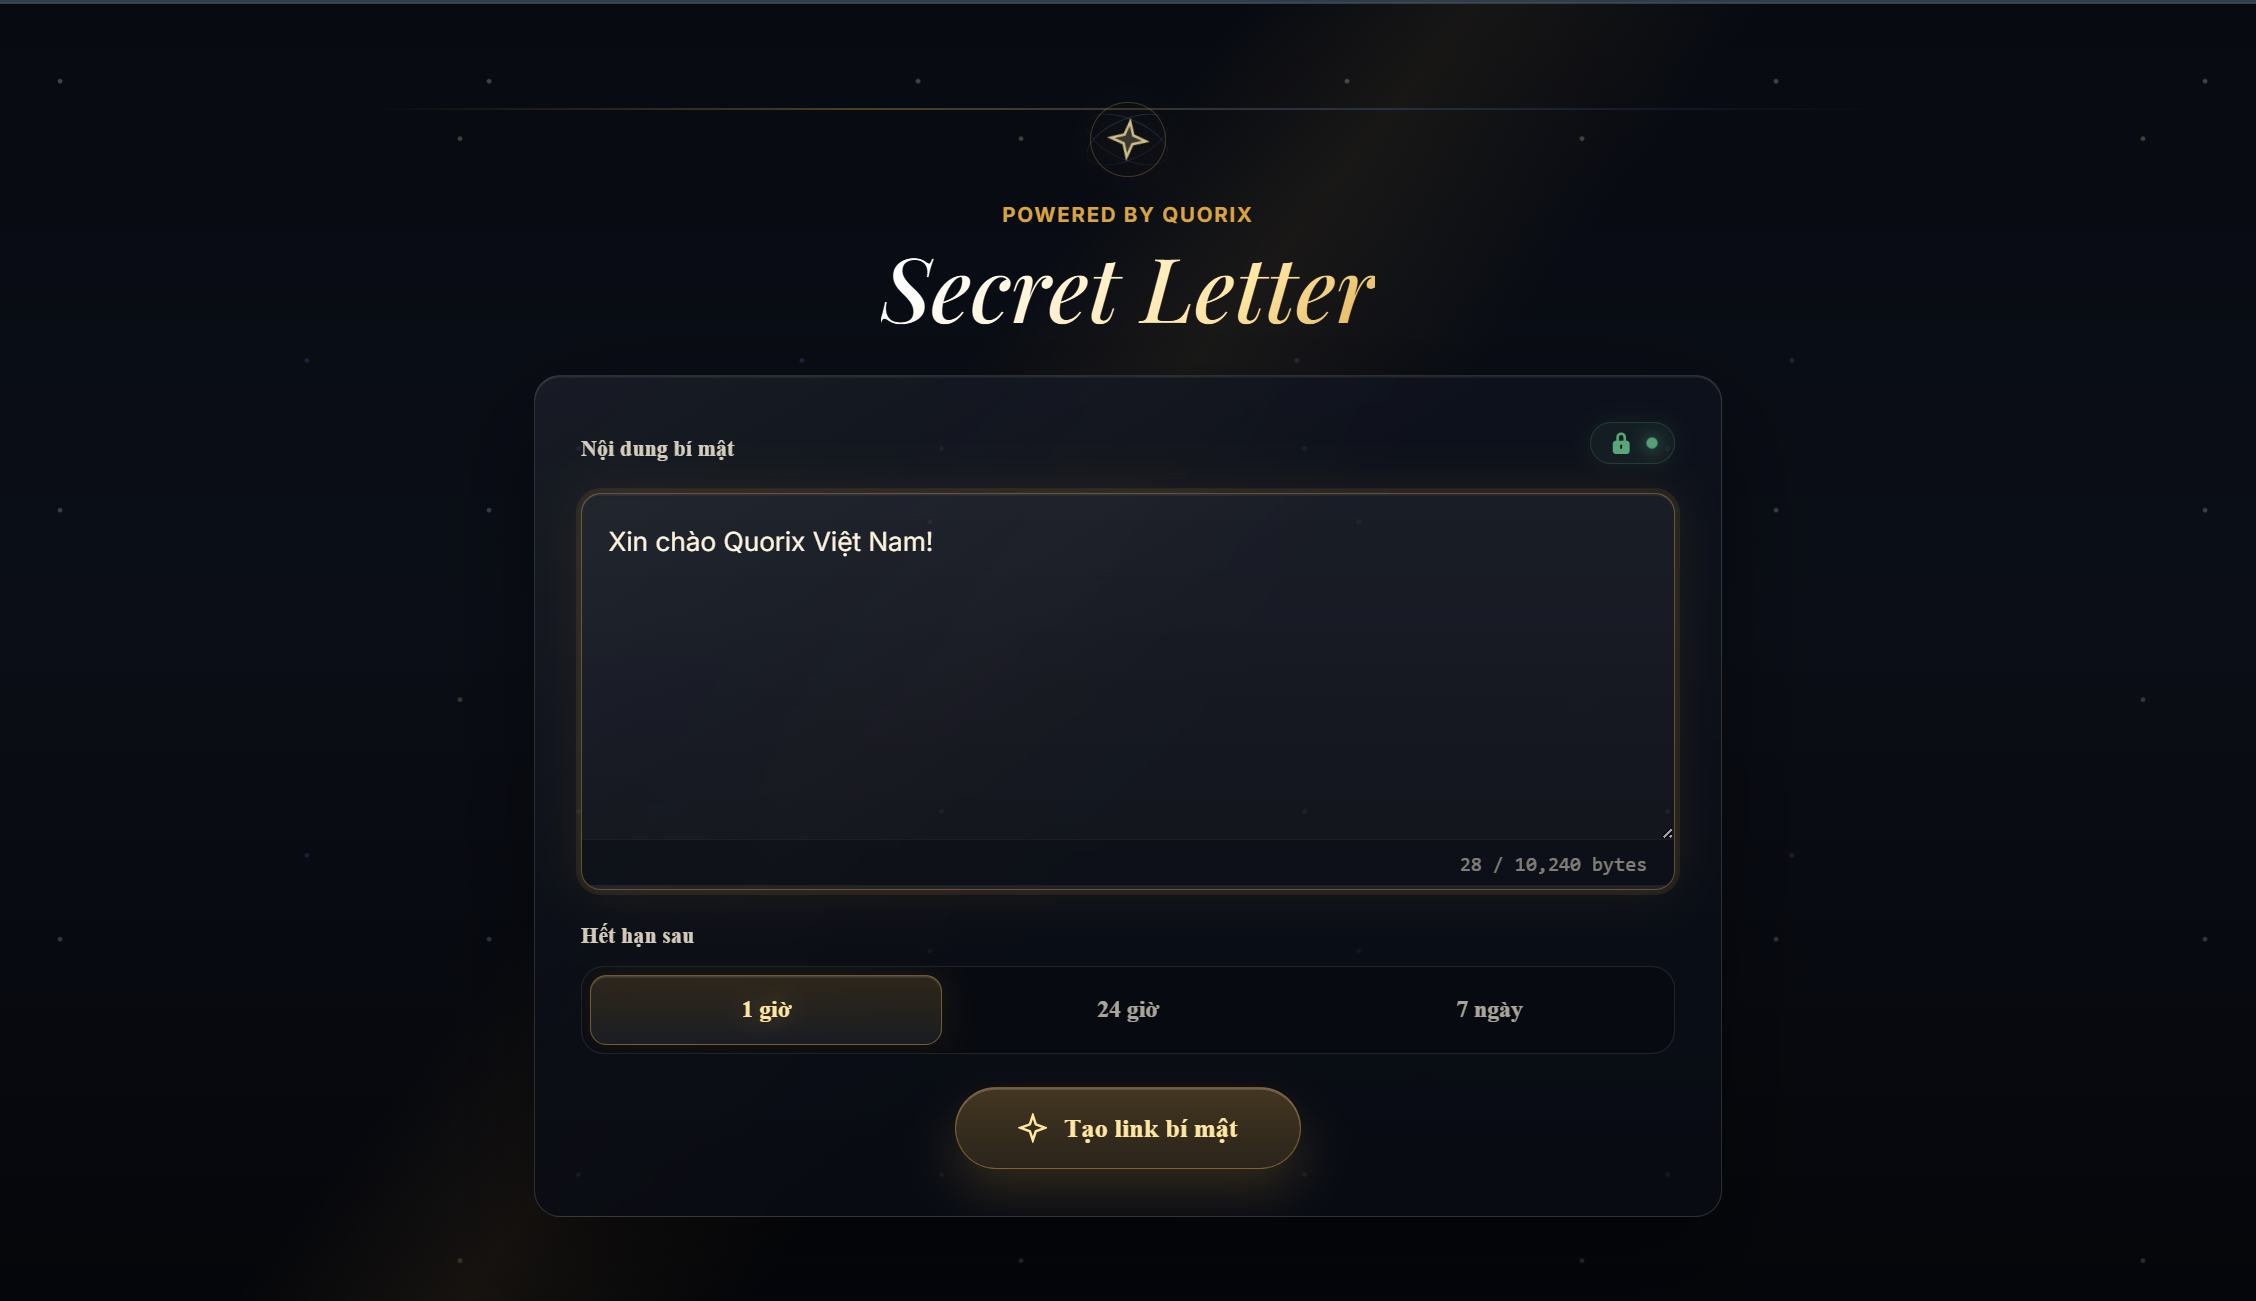
\includegraphics[width=0.8\textwidth]{img/ui_home_create.png}
        \caption[Giao diện soạn thảo thông điệp và cấu hình TTL]{Giao diện soạn thảo thông điệp và cấu hình thời gian sống (TTL)}
        \label{fig:ui_home_create}
    \end{figure}
    
    Khi người dùng tiến hành mã hóa, Frontend sẽ gọi API \texttt{POST /api/secrets} và chỉ cấp phát liên kết an toàn (Secret Link) khi máy chủ đã xác nhận lưu trữ bản mã thành công.

    \begin{figure}[H]
        \centering
        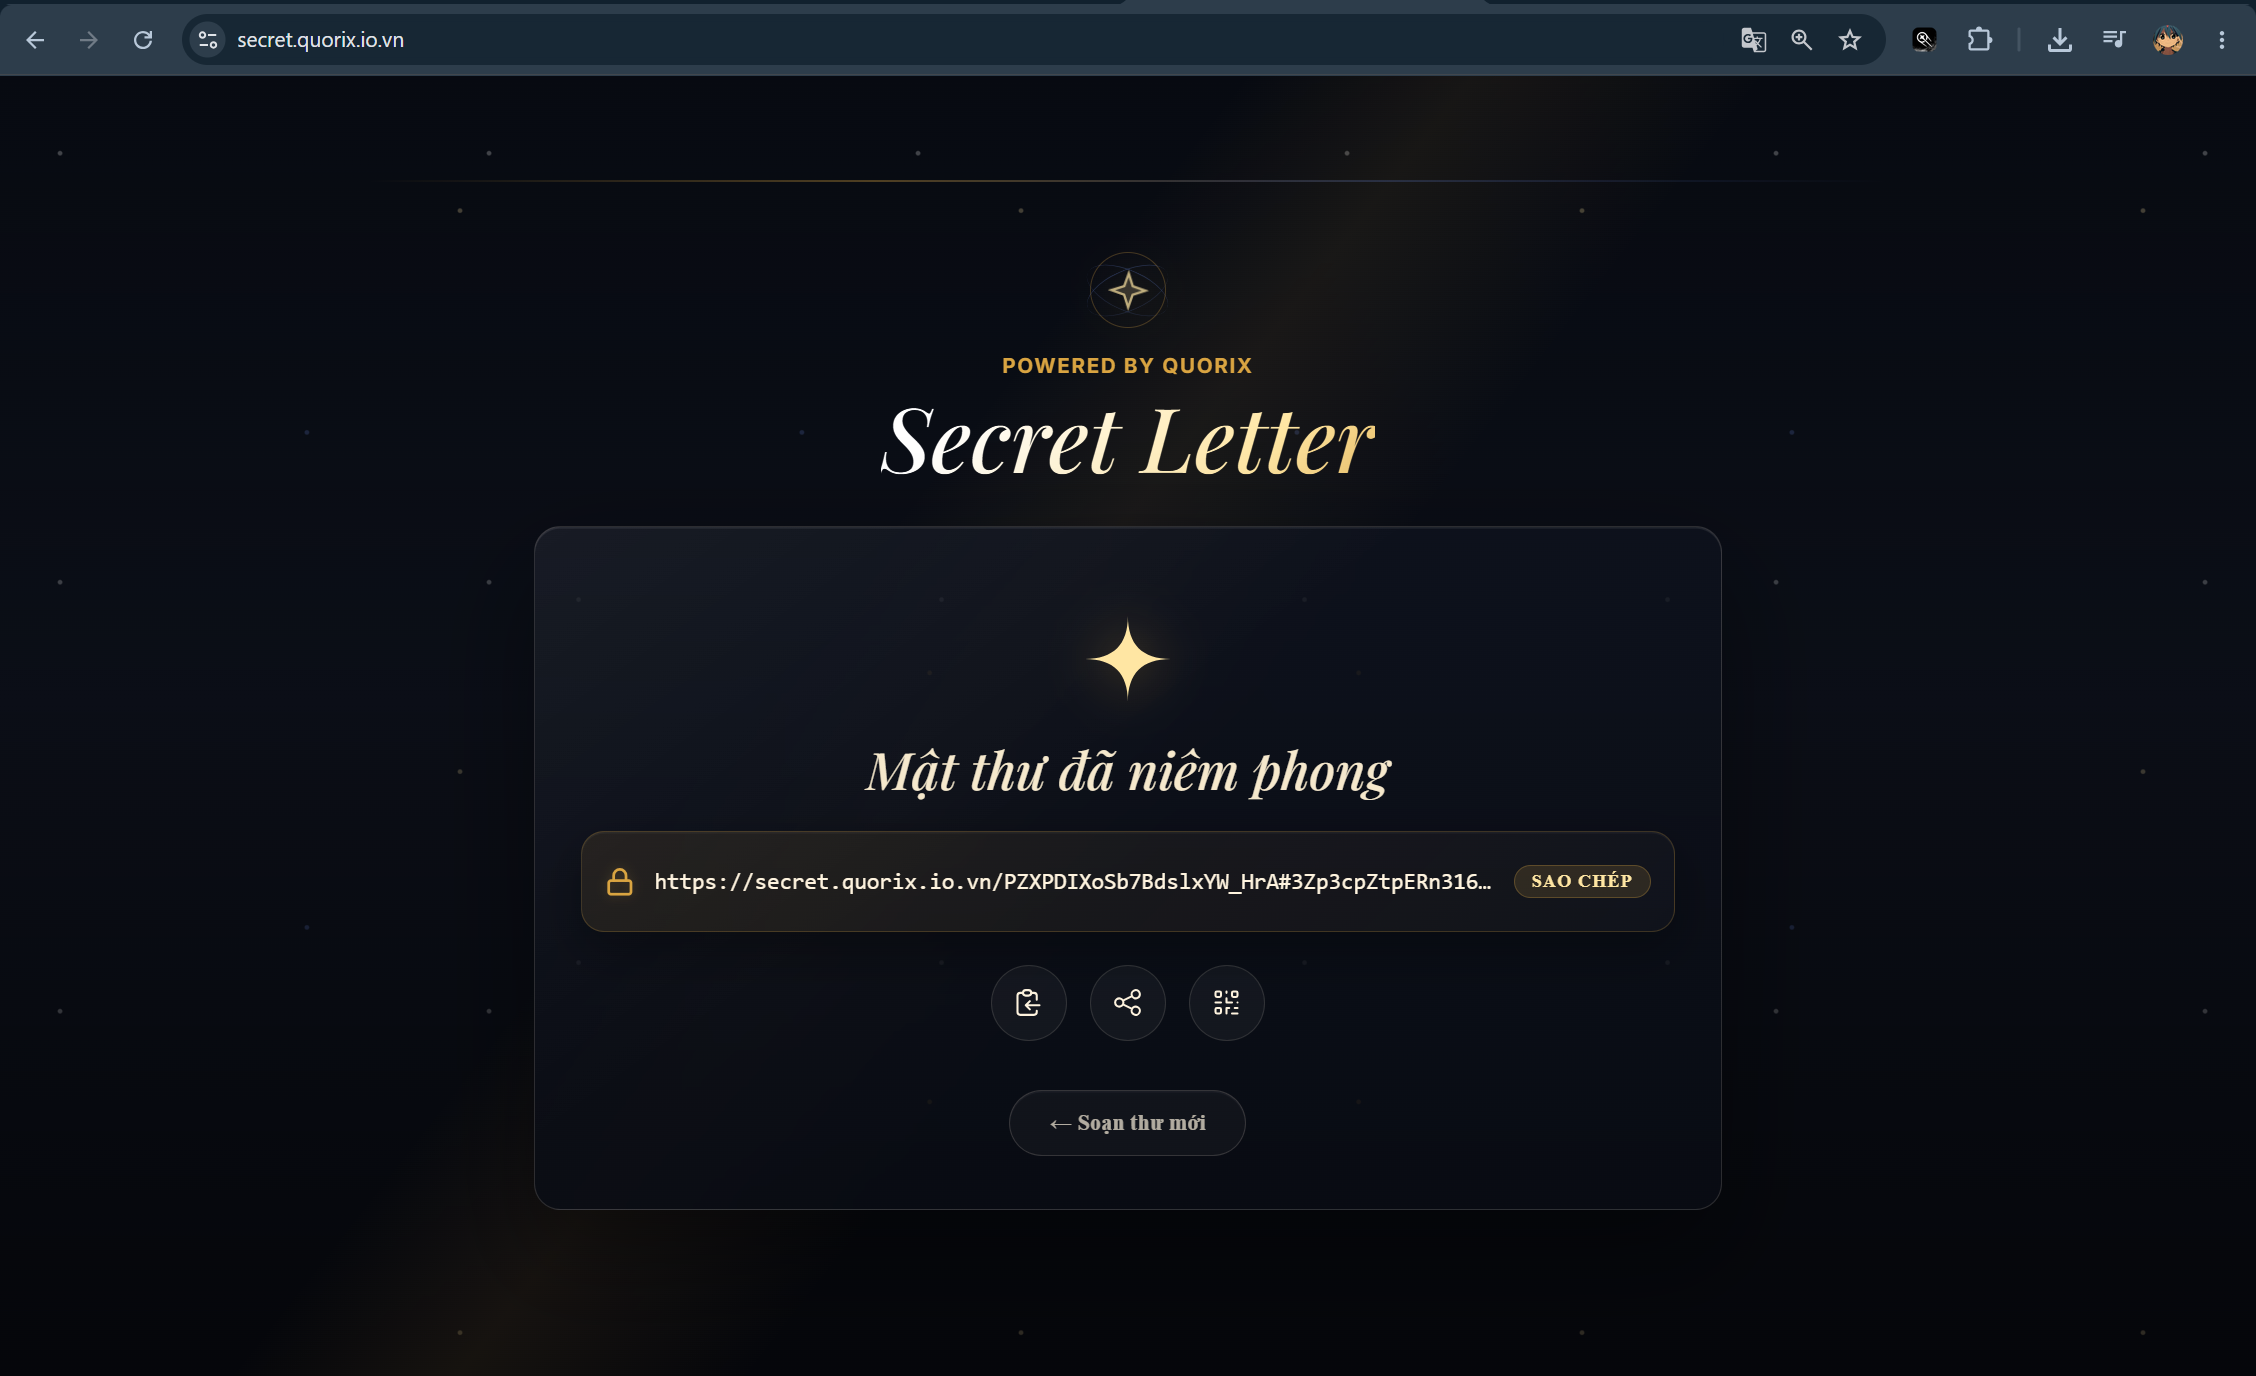
\includegraphics[width=0.8\textwidth]{img/ui_home_link.png}
        \caption[Trạng thái liên kết an toàn sau mã hóa]{Trạng thái trả về liên kết an toàn sau khi mã hóa thành công}
        \label{fig:ui_home_link}
    \end{figure}

    \item \textbf{RevealPage (Màn hình Giải mã):} Đảm nhận luồng kiểm duyệt và chống tự động hóa (Anti-Bot). Khi người nhận truy cập thông qua liên kết (chứa khóa giải mã tại đoạn \texttt{\#key=...}), hệ thống không tự ý tải bản mã về. Thay vào đó, giao diện sẽ thiết lập một phiên giao dịch ngắn hạn (Reveal Session) và yêu cầu người dùng thao tác vật lý (nhấn nút "Mở thư"). 

    \begin{figure}[H]
        \centering
        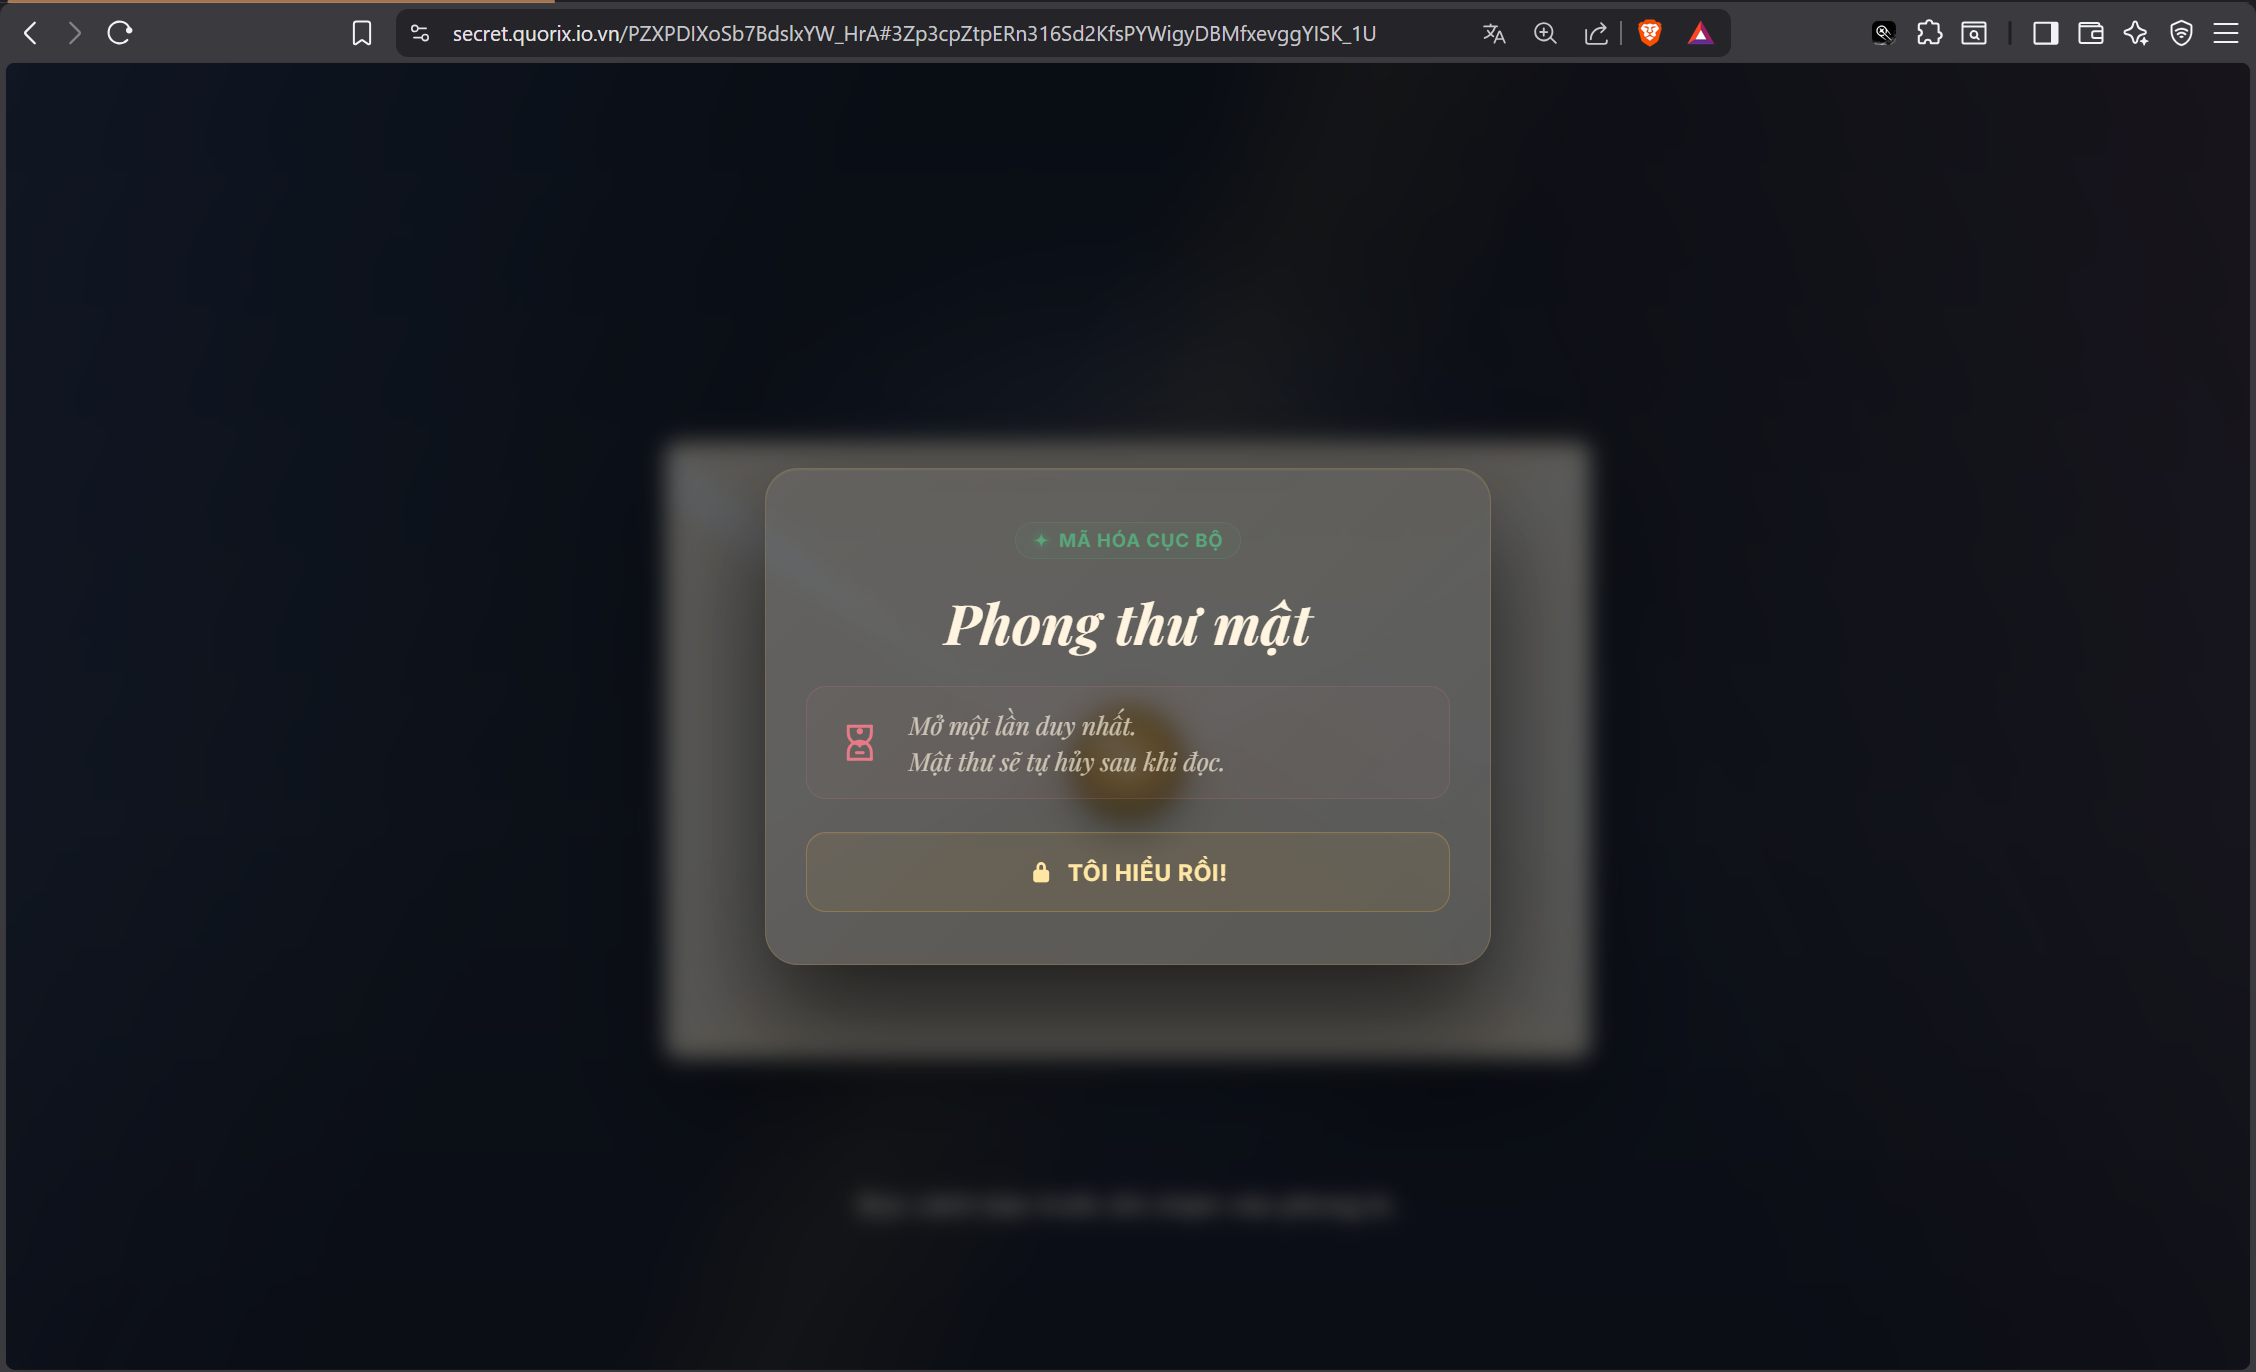
\includegraphics[width=0.8\textwidth]{img/ui_reveal_gate.png}
        \caption[Giao diện Anti-Bot xác thực tương tác vật lý]{Giao diện Anti-Bot buộc người nhận phải tương tác vật lý}
        \label{fig:ui_reveal_gate}
    \end{figure}

    Chỉ sau khi vượt qua rào cản này, văn bản mã hóa mới được trích xuất từ Redis, trả về trình duyệt và phục hồi thông qua hàm \texttt{decryptSecret}.

    \begin{figure}[H]
        \centering
        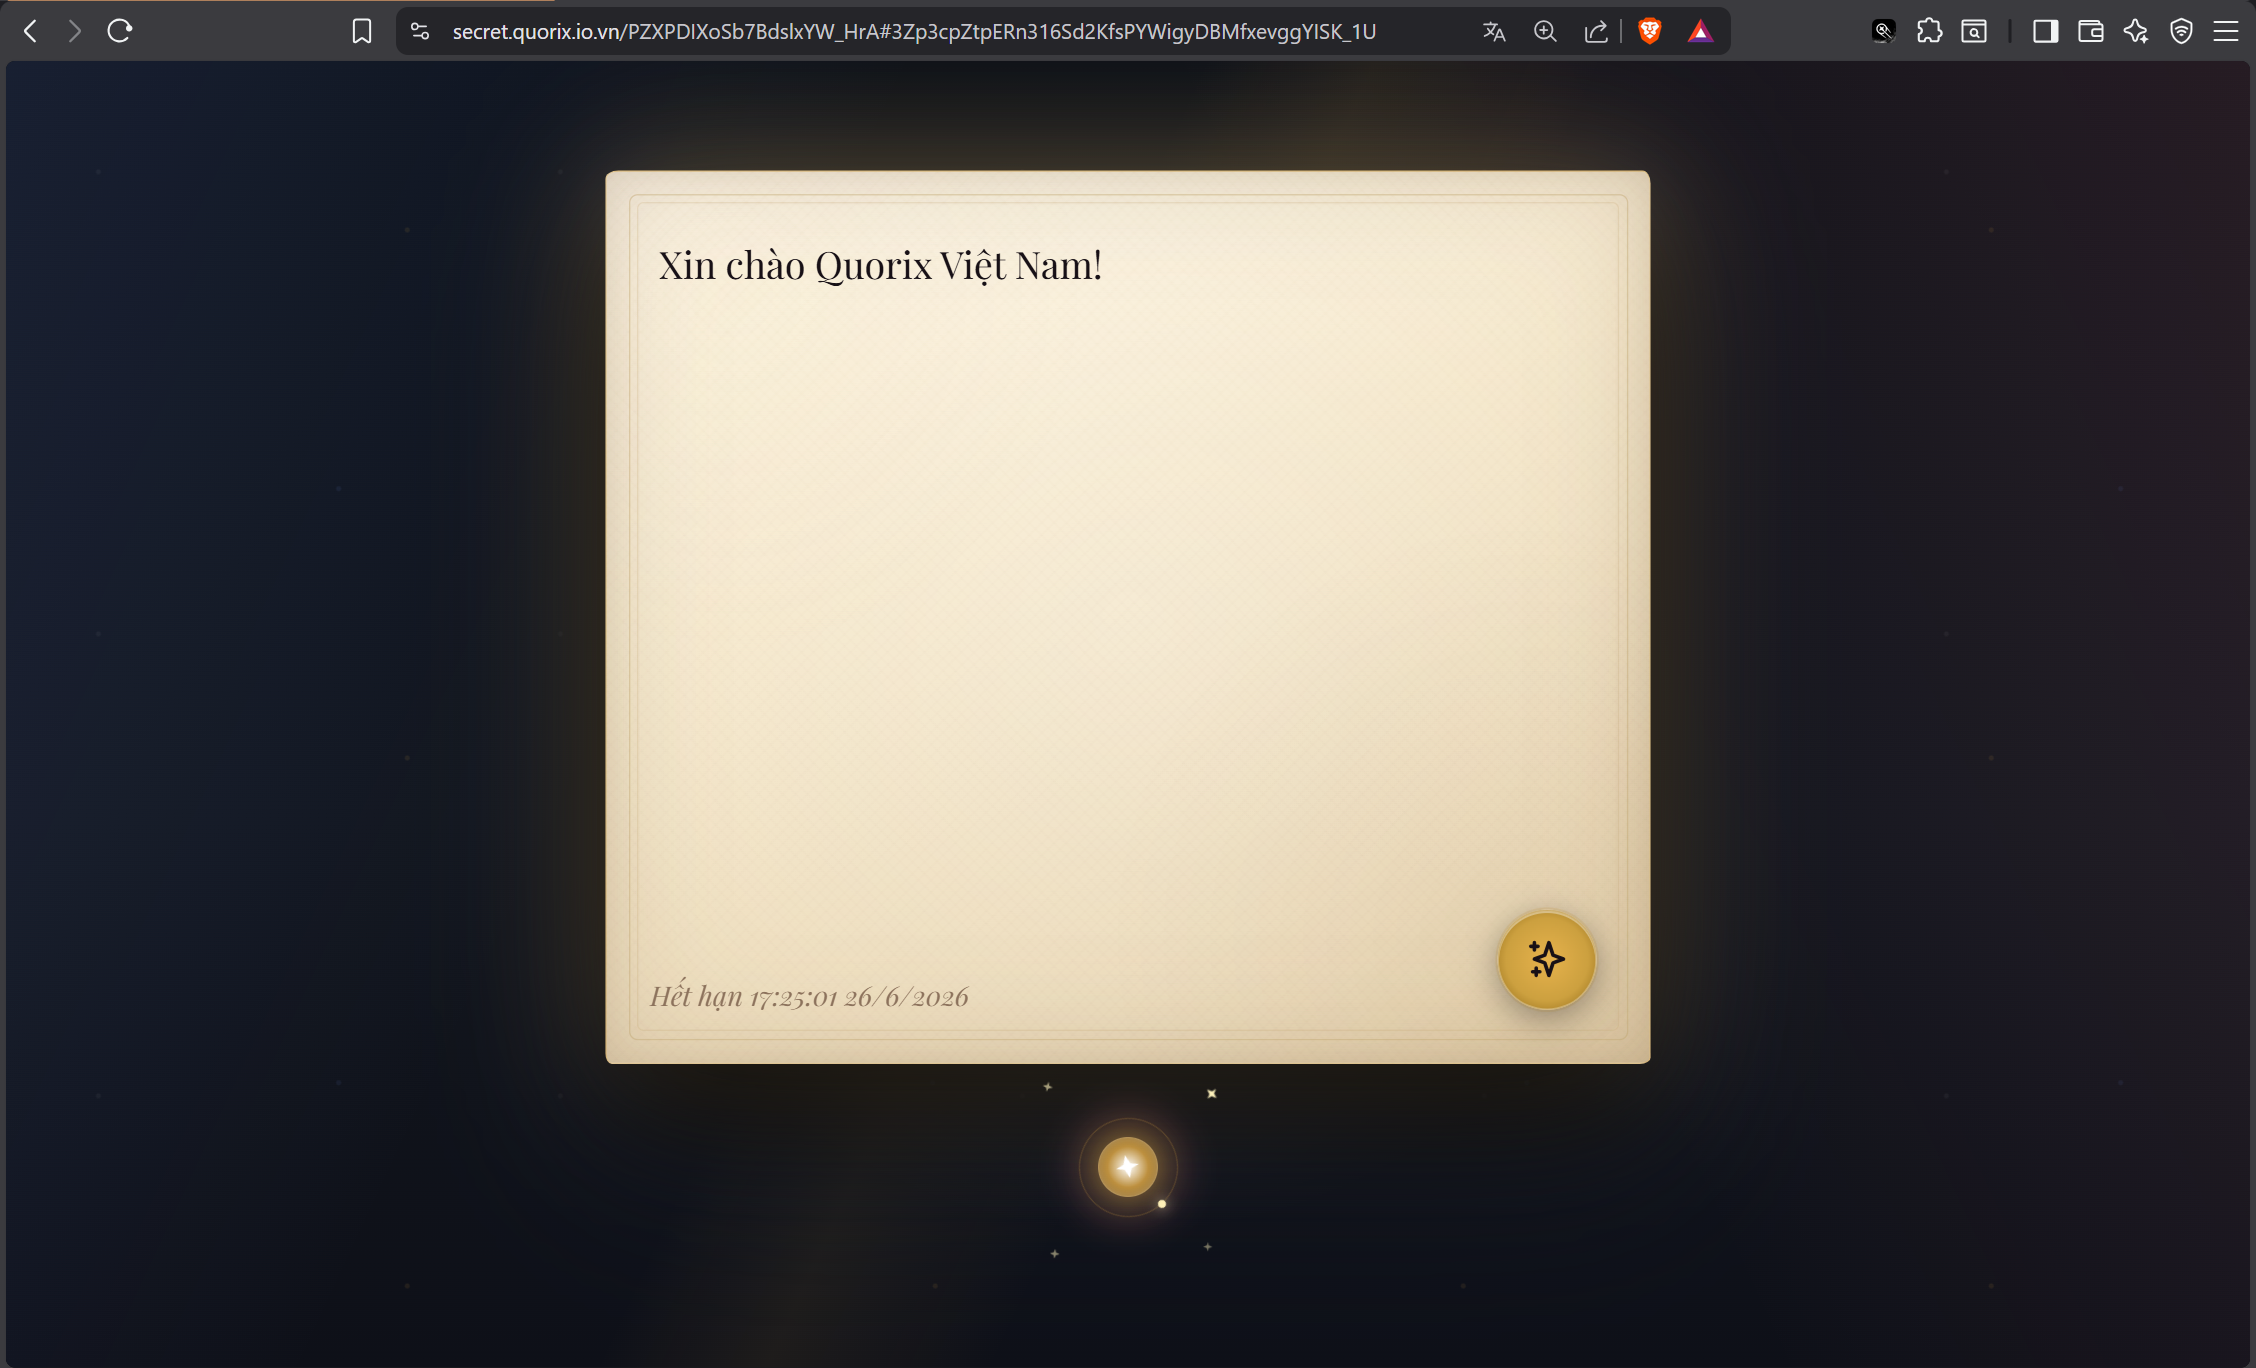
\includegraphics[width=0.8\textwidth]{img/ui_reveal_decrypted.png}
        \caption[Giao diện hiển thị nội dung thông điệp sau giải mã]{Giao diện hiển thị nội dung thông điệp sau khi giải mã thành công}
        \label{fig:ui_reveal_decrypted}
    \end{figure}

    Ngay sau khi thông điệp được giải mã và hiển thị, bản ghi trên máy chủ Redis sẽ lập tức bị xóa bỏ. Nếu người dùng vô tình tải lại trang hoặc truy cập lại liên kết, hệ thống sẽ thông báo lá thư đã bị tiêu hủy, hoàn tất vòng đời "Burn-after-reading" (Hình \ref{fig:ui_reveal_destroyed}).

    \begin{figure}[H]
        \centering
        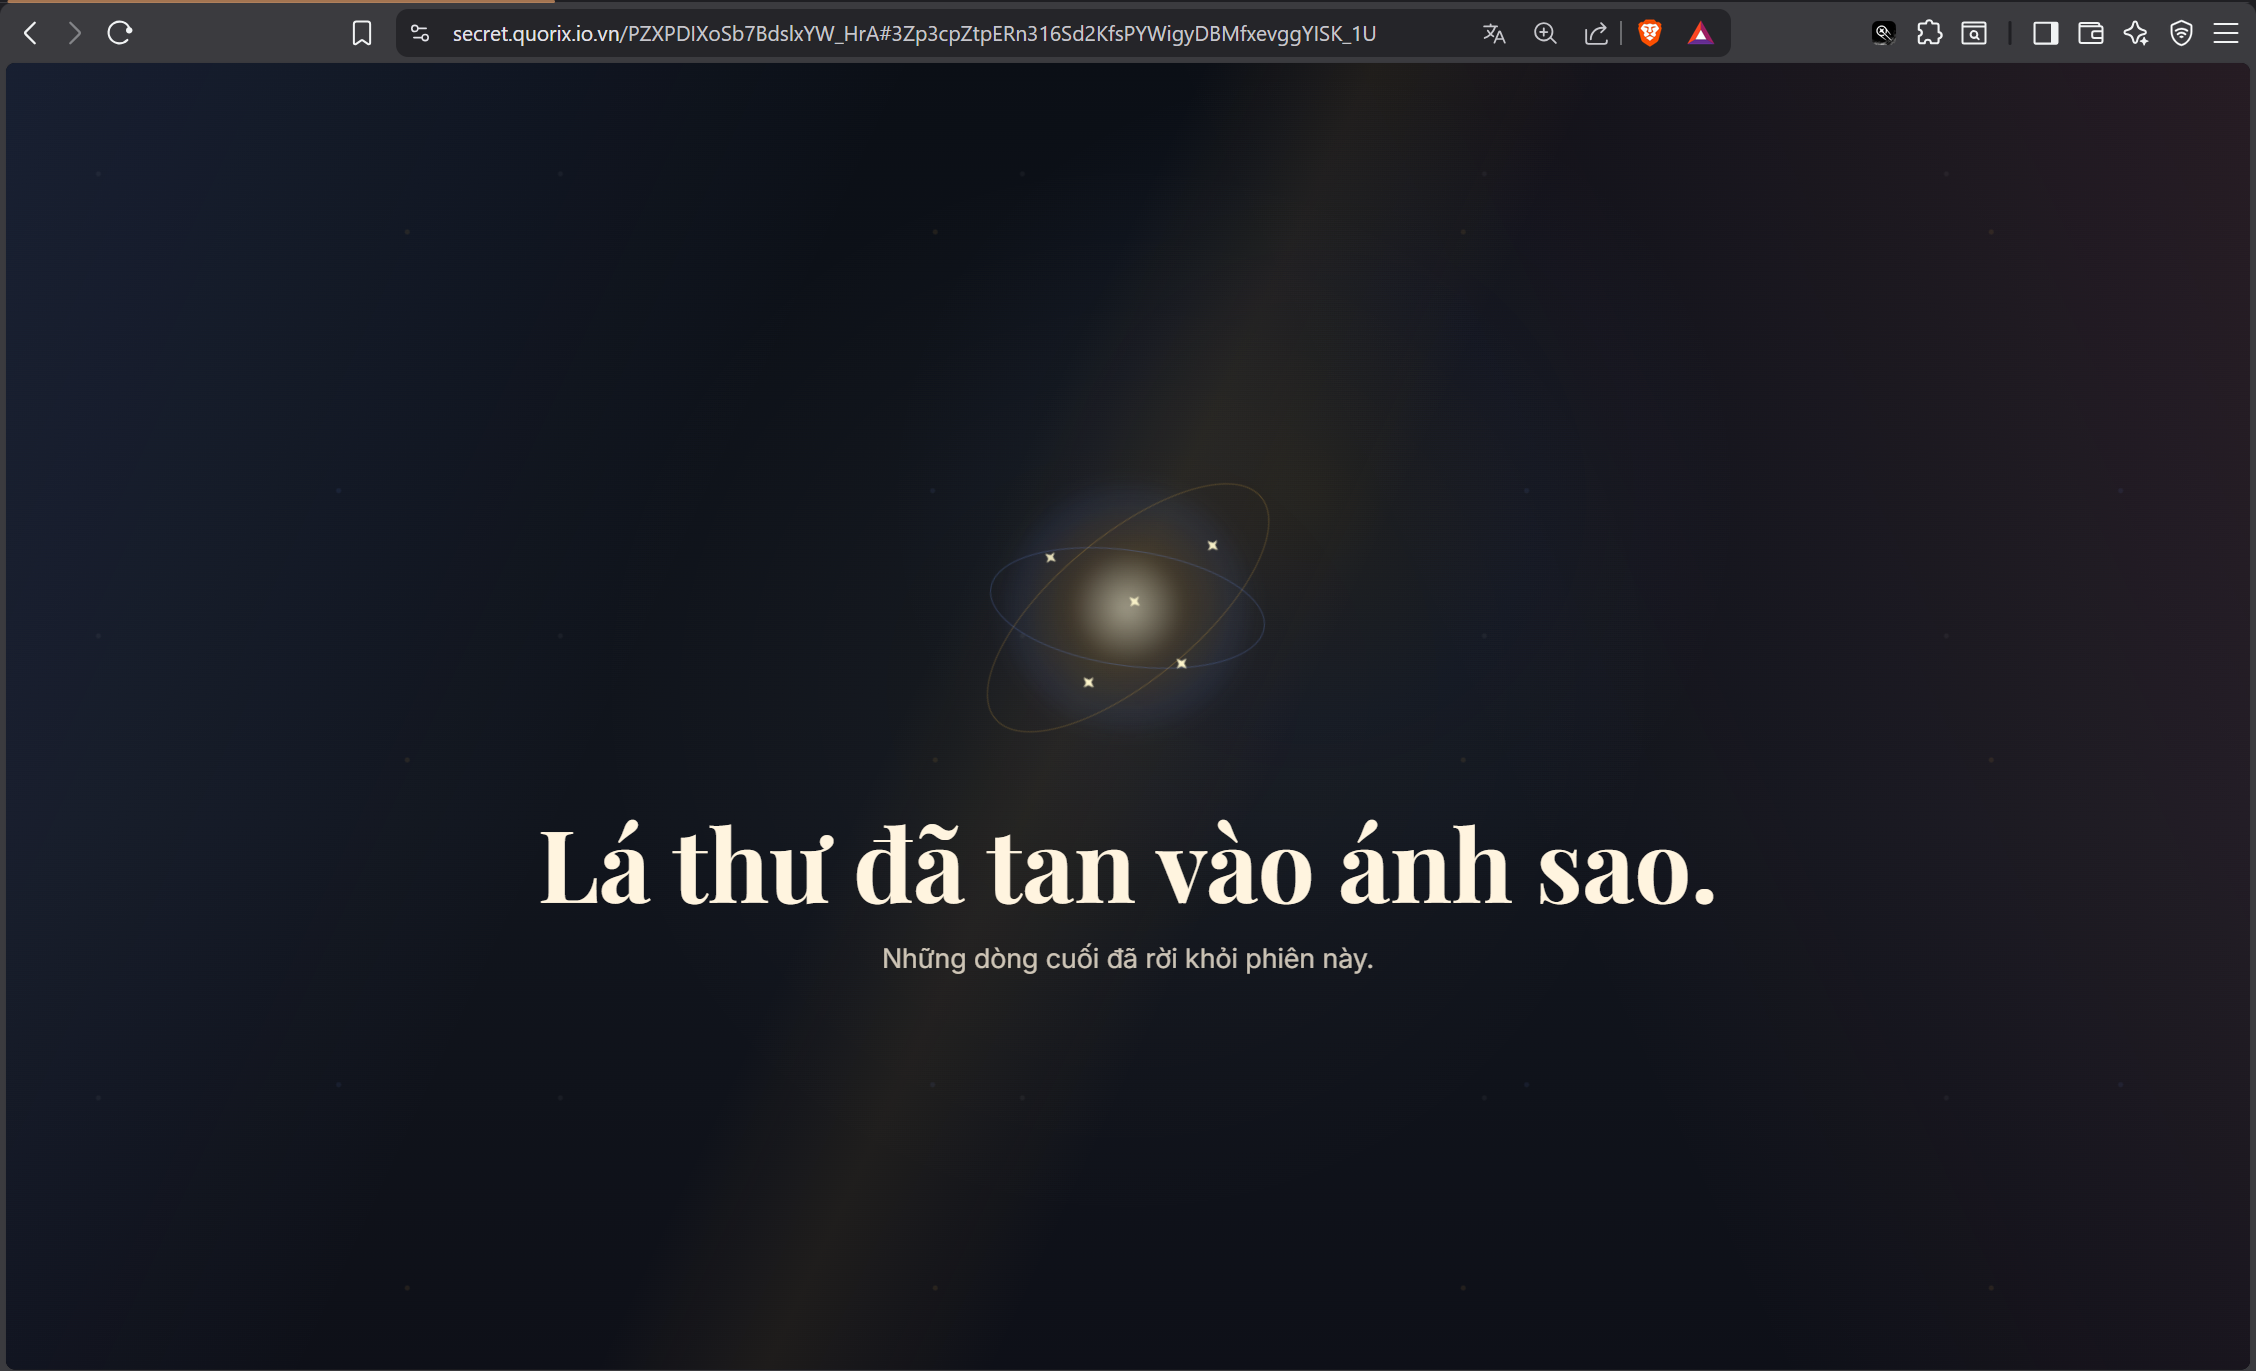
\includegraphics[width=0.8\textwidth]{img/ui_reveal_destroyed.png}
        \caption[Giao diện thông báo thư bị hủy vĩnh viễn]{Giao diện thông báo lá thư đã bị huỷ vĩnh viễn}
        \label{fig:ui_reveal_destroyed}
    \end{figure}

    \item \textbf{Xử lý ngoại lệ (Error Boundaries):} Nhằm đảm bảo trải nghiệm người dùng, Frontend cung cấp các phản hồi thị giác rõ ràng khi luồng giải mã gặp sự cố. Điển hình là việc nhận diện các truy cập thiếu tham số khóa mã hóa (Missing Key), hoặc khóa không hợp lệ (Wrong Key) dẫn đến thất bại trong việc giải mã.

    \begin{figure}[H]
        \centering
        \begin{minipage}{0.48\textwidth}
            \centering
            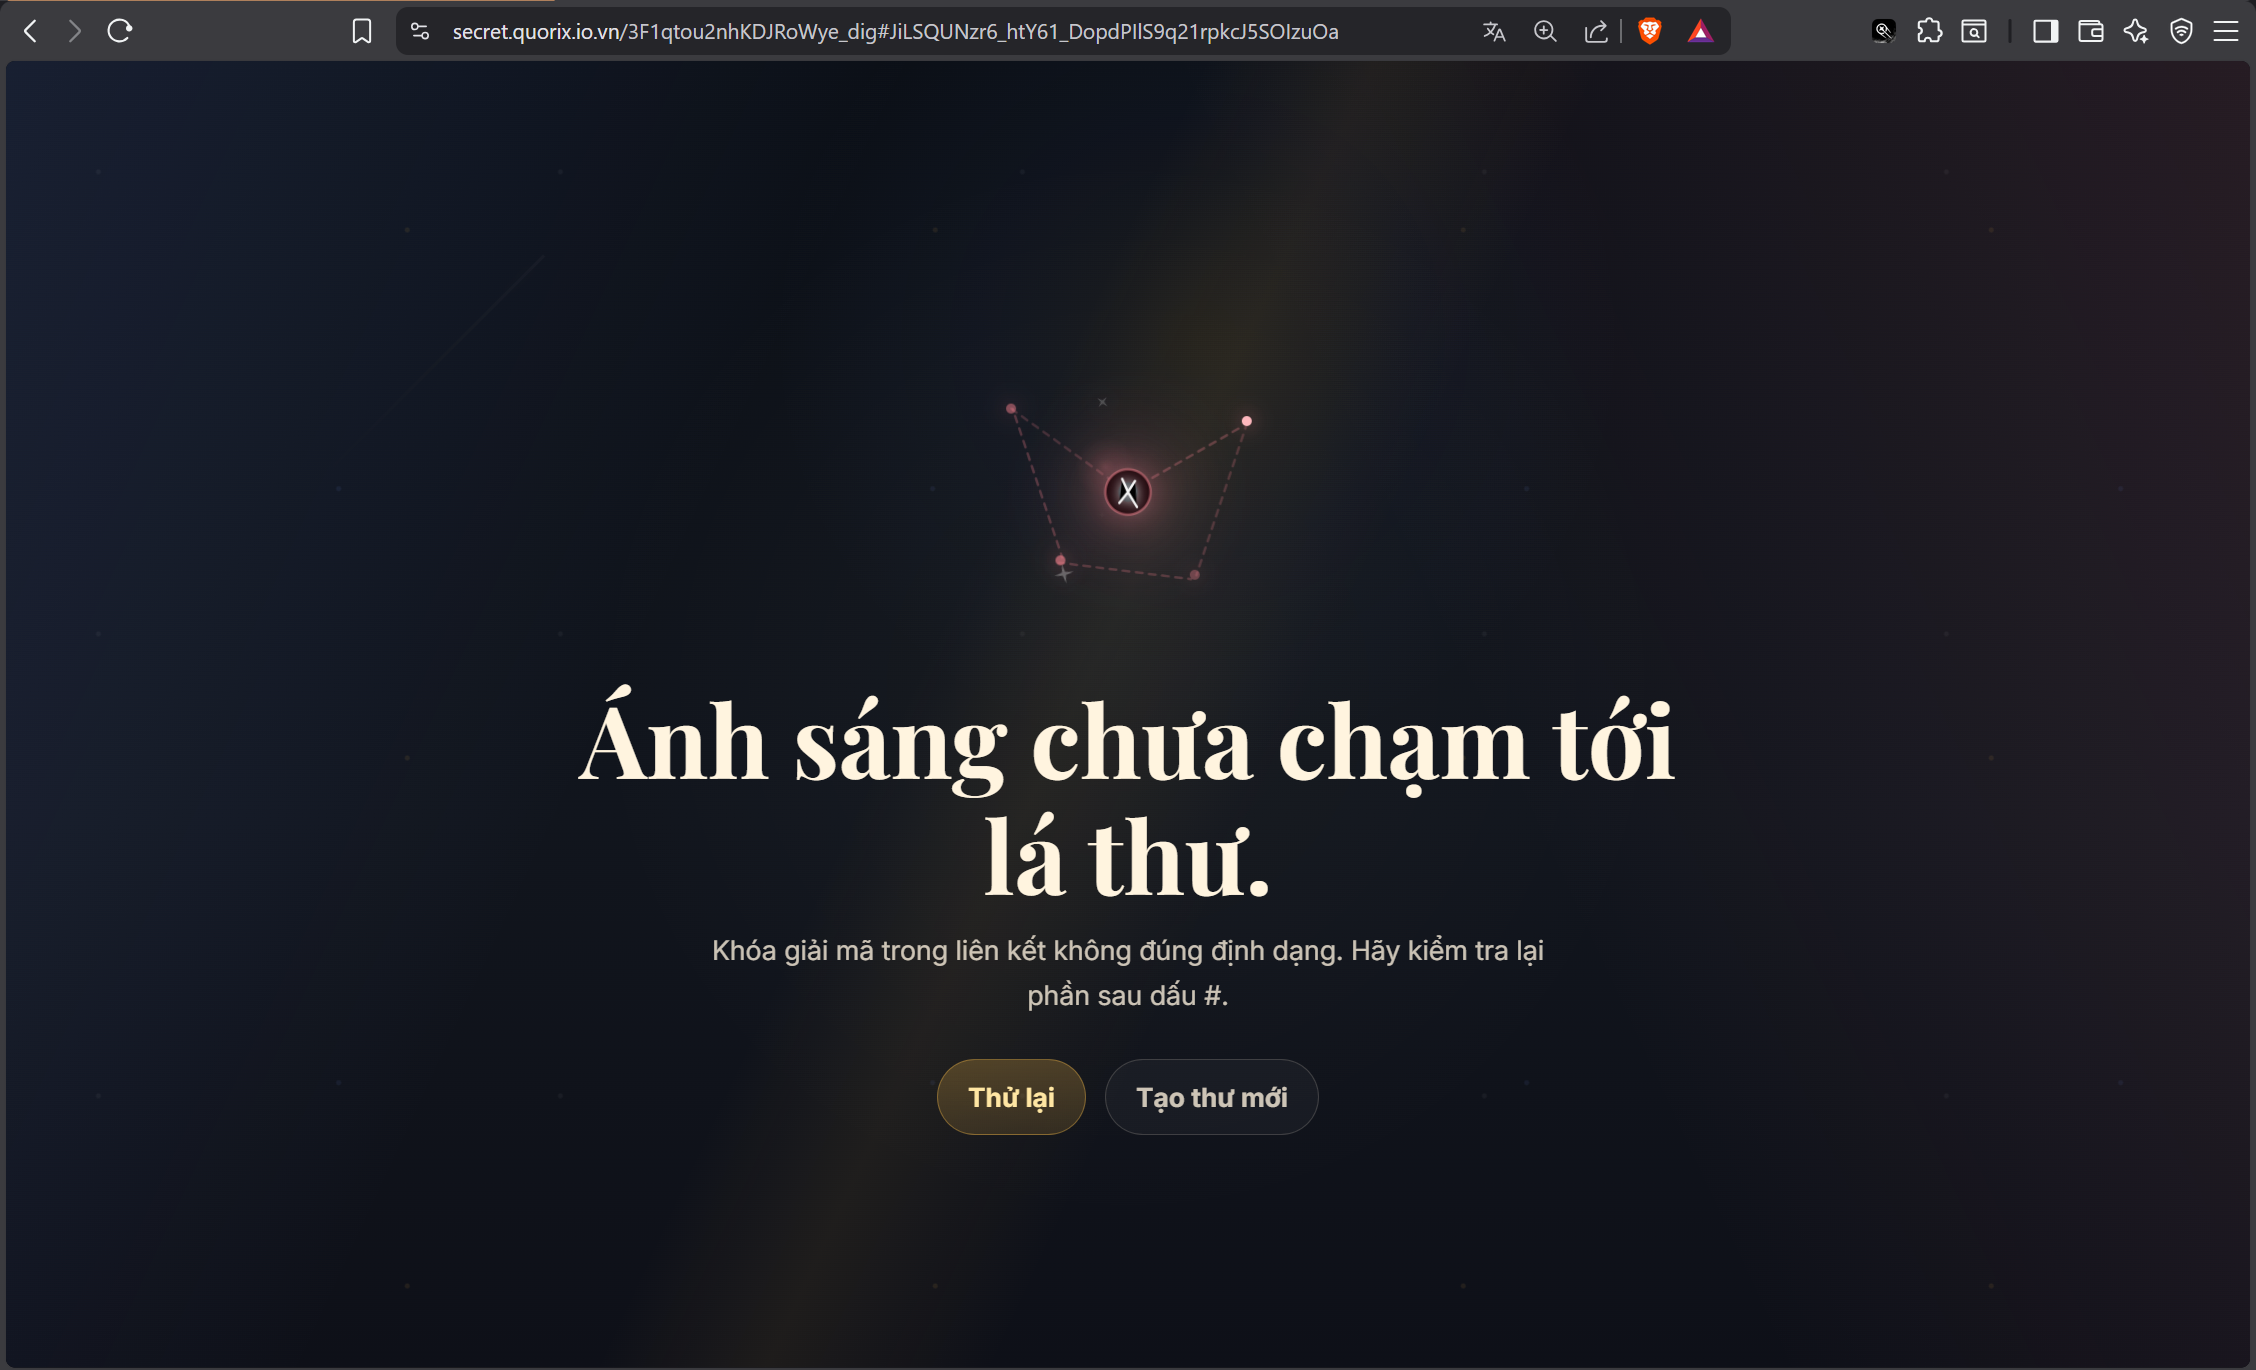
\includegraphics[width=\linewidth]{img/ui_error_nokey.png}
            \caption[Cảnh báo khi liên kết thiếu đoạn khóa]{Cảnh báo khi liên kết thiếu đoạn khóa}
            \label{fig:ui_error_nokey}
        \end{minipage}\hfill
        \begin{minipage}{0.48\textwidth}
            \centering
            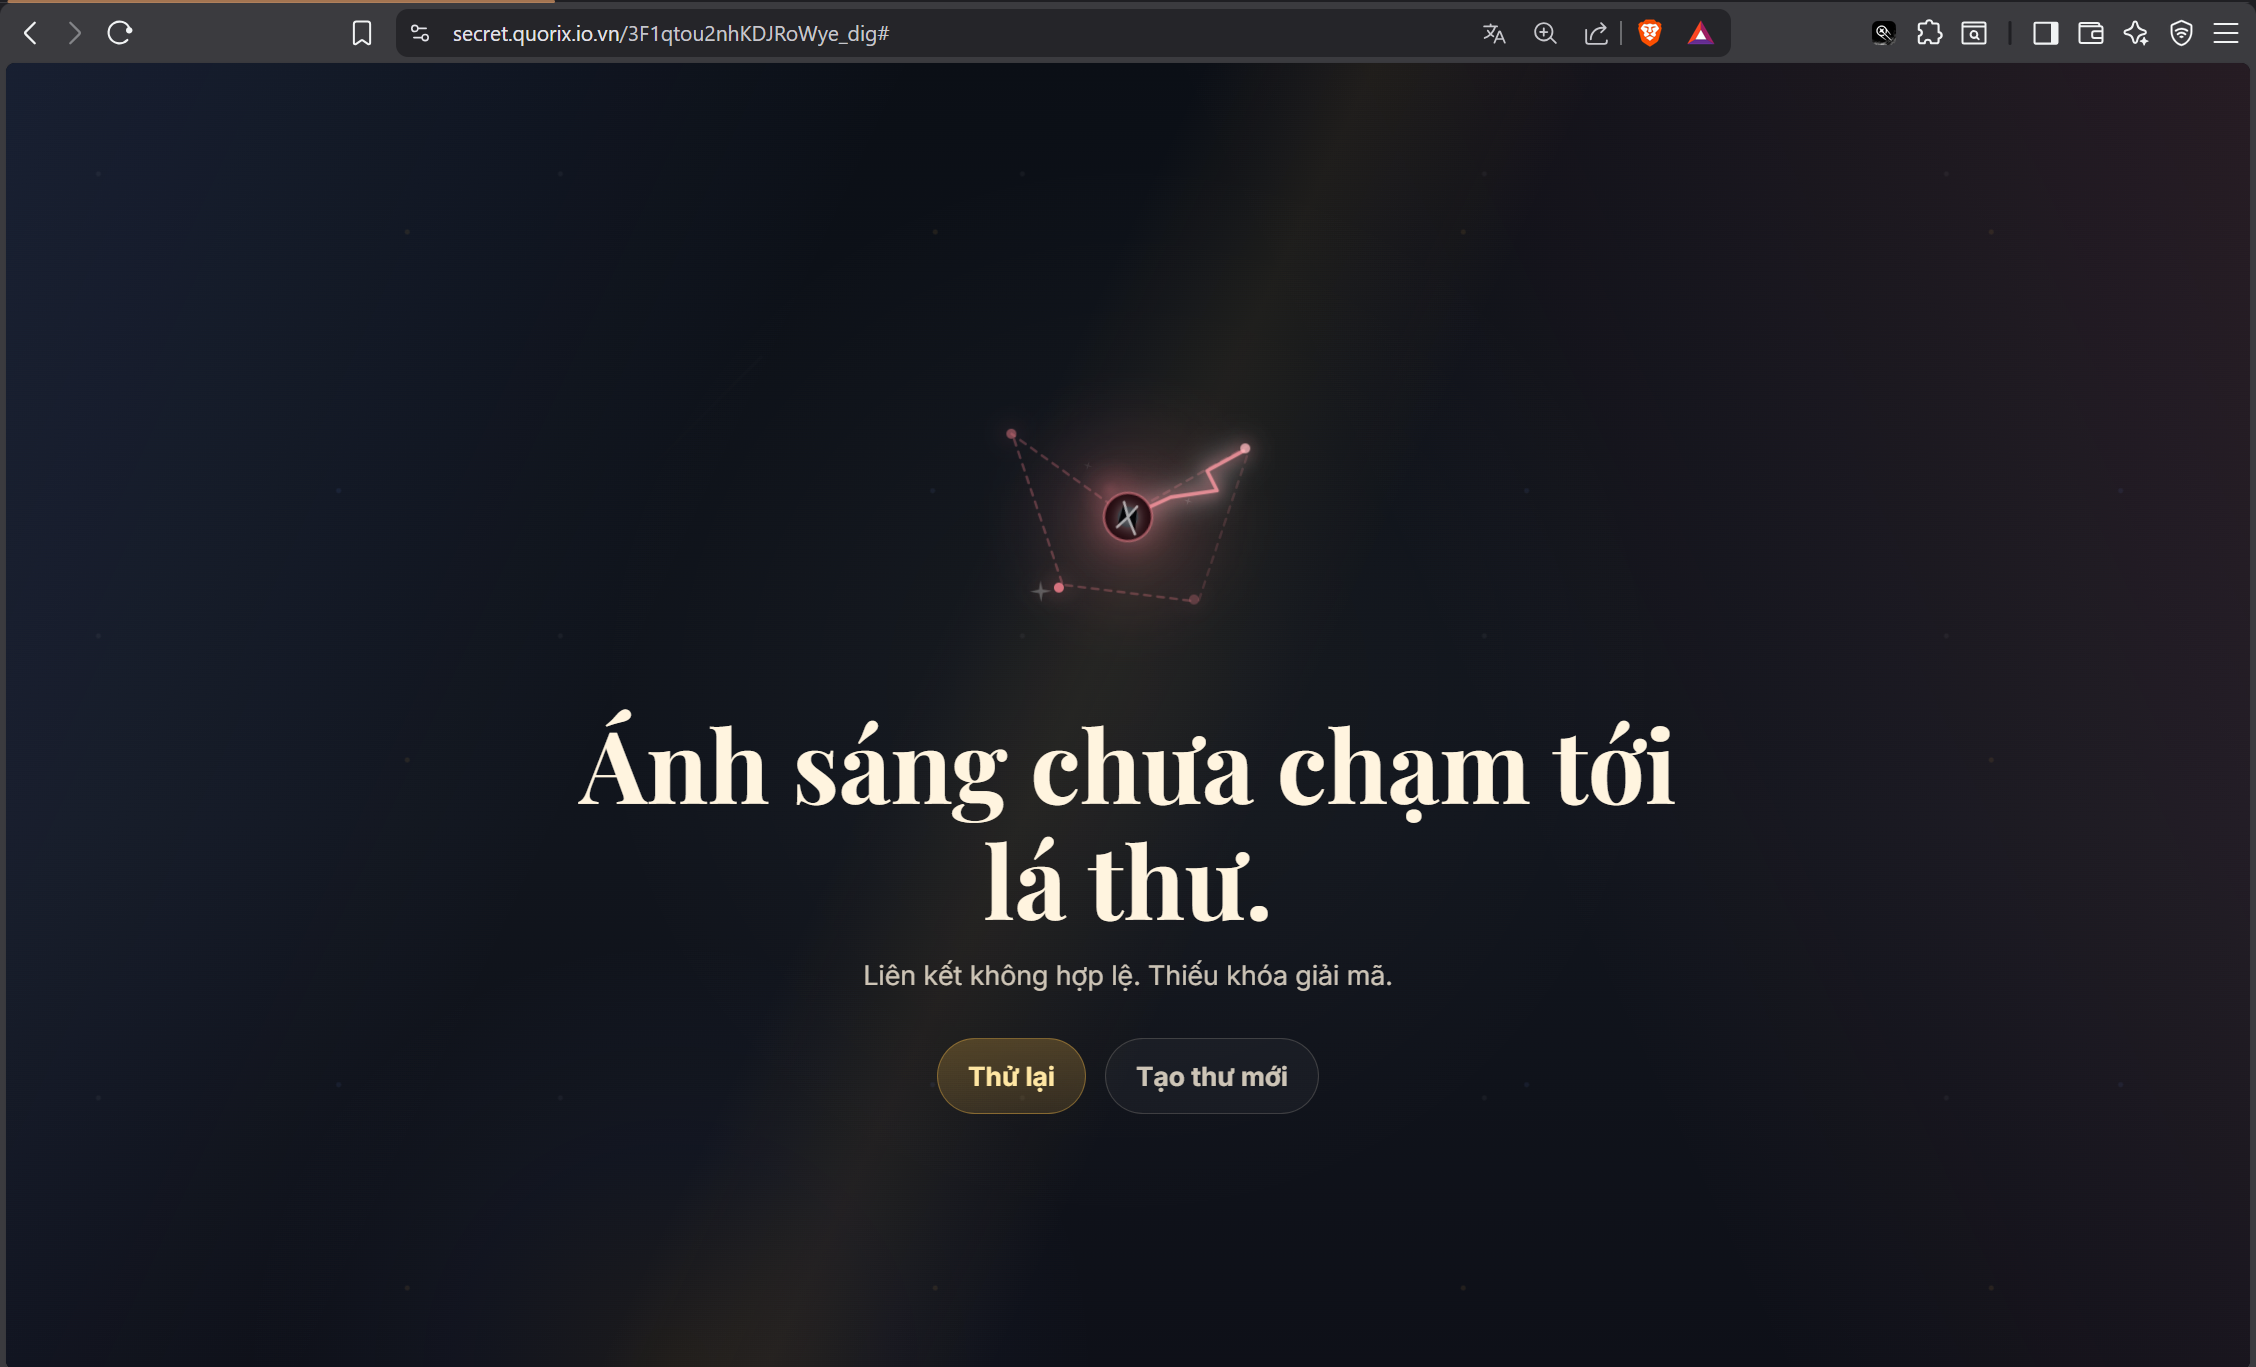
\includegraphics[width=\linewidth]{img/ui_error_wrongkey.png}
            \caption[Cảnh báo khi giải mã thất bại do sai khóa]{Cảnh báo khi giải mã thất bại do sai khóa}
            \label{fig:ui_error_wrongkey}
        \end{minipage}
    \end{figure}
\end{itemize}
\section{Triển khai Backend}

Phân hệ máy chủ (Backend) của \textit{Secret Letter} được thiết kế với hai tiêu chí trọng tâm: Tốc độ phản hồi cực nhanh (Low Latency) và độ tin cậy cao trong quá trình tiêu hủy dữ liệu.

\subsection{Lựa chọn công nghệ cốt lõi}

\begin{itemize}
    \item \textbf{Ngôn ngữ Golang:} Được lựa chọn nhờ khả năng xử lý đồng thời (Concurrency) ưu việt thông qua Goroutines, kết hợp với lợi thế biên dịch ra tệp thực thi độc lập (Standalone Binary). Điều này giúp tối giản hóa quá trình triển khai nền tảng đám mây, hạn chế tối đa sự phụ thuộc vào các môi trường thực thi cồng kềnh (như JVM hay Node.js).
    \item \textbf{Cơ sở dữ liệu Redis:} Thay vì sử dụng các cơ sở dữ liệu quan hệ (RDBMS) lưu trữ trên ổ cứng vật lý, Redis (In-Memory Database) được ưu tiên để quản lý thông điệp. Với cơ chế ghi nhận bộ nhớ tạm và tự động thu hồi dựa trên thời gian sống (TTL - Time to Live) tích hợp sẵn, Redis là mảnh ghép cực kỳ phù hợp cho cấu trúc đọc-một-lần (Burn-after-reading).
\end{itemize}

\subsection{Kiểm soát tính nguyên tử (Atomic Operations)}

Một trong những bài toán bảo mật phức tạp tại Backend là rủi ro tương tranh (Race Condition), nơi nhiều luồng kết nối mạng đồng loạt gửi yêu cầu mở cùng một bức thư. Nếu không được rào chắn, dữ liệu có thể vô tình bị trích xuất làm nhiều bản.

Để giải quyết, tầng nghiệp vụ lưu trữ (thuộc \texttt{internal/\-secret/\-redis\_service.go}) đã áp dụng các kịch bản \textbf{Lua Script} thực thi trực tiếp trên Redis Engine. Lợi dụng bản chất tiến trình đơn luồng (Single-threaded) của hệ thống Redis, toàn bộ chuỗi thao tác: Kiểm tra sự tồn tại $\rightarrow$ Trích xuất bản mã $\rightarrow$ Xóa sổ vật lý (DEL) được thi hành dưới dạng một giao dịch nguyên tử (Atomic Transaction) không thể chia cắt. Cơ chế này đóng vai trò quyết định trong việc ngăn ngừa hiệu quả mọi nỗ lực lợi dụng độ trễ mạng để tải xuống bức thư lần thứ hai.

\subsection{Hệ thống giới hạn lưu lượng (Rate Limiting)}

Nhằm bảo vệ tài nguyên máy chủ trước các nguy cơ tấn công làm cạn kiệt dịch vụ (DoS) hoặc bơm dữ liệu rác làm tràn bộ nhớ, cơ chế Rate Limiting độc lập đã được xây dựng chuyên biệt tại phân vùng \texttt{internal/\-ratelimit}.

Thuật toán đếm cửa sổ cố định (Fixed Window Counter) cũng được triển khai qua Lua Script nhằm đạt tốc độ đánh giá nhanh nhất. Hệ thống thiết lập các ranh giới khắt khe để duy trì tính ổn định:
\begin{itemize}
    \item Tối đa \textbf{120 lần} khởi tạo thư (\texttt{Create}) / giờ / IP.
    \item Tối đa \textbf{240 lần} mở thư (\texttt{Consume}) / giờ / IP.
\end{itemize}

Nhằm nâng cao tính ẩn danh, hệ thống chỉ lưu trữ mã băm (Hash) theo chuẩn SHA-256 của địa chỉ IP để làm khóa đếm giới hạn (Rate Limit Key) trong Redis, đảm bảo hệ thống không lưu giữ vết tích mạng thực tế của người dùng.

\subsection{Phân lớp kiến trúc và Xử lý lỗi}

Kiến trúc phần mềm được phân rã thành ba tầng trừu tượng chính:
\begin{enumerate}
    \item \textbf{Tầng Mạng (\texttt{httpapi}):} Quản lý việc tiếp nhận yêu cầu, thiết lập các lớp lá chắn bảo mật biên (CORS, Security Headers, Max Payload Size) và chuẩn hóa dữ liệu đầu vào.
    \item \textbf{Tầng Nghiệp vụ (\texttt{secret}):} Kiểm soát vòng đời cấp phát phiên giao dịch (Reveal Session) và đánh giá logic mã hóa (kiểm tra tính hợp lệ của chuẩn mã hóa, Nonce, TTL).
    \item \textbf{Tầng Dữ liệu (\texttt{store}):} Phụ trách kênh kết nối TCP tốc độ cao với máy chủ Redis.
\end{enumerate}

Bất kỳ sự cố nào phát sinh xuyên suốt cấu trúc ba tầng này đều được hệ thống quy hoạch về chuẩn lỗi nội bộ \texttt{AppError}. Cách tiếp cận này giúp Backend không bao giờ vô tình làm rò rỉ mã lỗi hệ thống (như Stacktrace hay Lỗi thư viện) ra bên ngoài, đồng thời đảm bảo Frontend luôn nhận được mã định danh sự cố (Error Codes) có ngữ nghĩa thống nhất.
\section{Giải quyết các bài toán kỹ thuật}

Quá trình phát triển \textit{Secret Letter} đòi hỏi sự kết hợp chặt chẽ giữa thiết kế hệ thống và nghiệp vụ mật mã học. Dưới đây là hai bài toán kỹ thuật then chốt và phương án giải quyết đã được áp dụng trong dự án.

\subsection{Bảo mật khóa giải mã trên đường truyền}

\textbf{Bài toán:} Mặc dù văn bản đã được mã hóa cục bộ tại Client (trình duyệt), khóa giải mã vẫn phải được chia sẻ từ người gửi đến người nhận. Nếu khóa này vô tình bị rò rỉ qua các tiêu đề giao thức (HTTP Headers), nhật ký truy cập (Access Logs) của máy chủ, hoặc các nút phân phối mạng trung gian (Proxy/Load Balancer), nguyên tắc Không tri thức (Zero-Knowledge) sẽ bị ảnh hưởng nghiêm trọng.

\textbf{Giải pháp:} Dự án khai thác một đặc tính cốt lõi của tiêu chuẩn web: \textbf{URL Fragment} (phần chuỗi ký tự nằm sau dấu \texttt{\#}).
Theo tiêu chuẩn RFC 3986, các trình duyệt web hiện đại có cơ chế giữ lại toàn bộ URL Fragment ở phía thiết bị người dùng và mặc định không đính kèm đoạn dữ liệu này vào các gói tin HTTP gửi lên máy chủ. Định dạng liên kết bí mật được thiết kế dưới dạng:
\begin{center}
    \texttt{https://domain/[ID]\#[Khoa\_Giai\_Ma]}
\end{center}
Nhờ vậy, khi người nhận truy cập liên kết, máy chủ Backend chỉ nhận được \texttt{[ID]} để tiến hành truy xuất bản mã, trong khi \texttt{[Khoa\_Giai\_Ma]} vẫn nằm lại an toàn trên thanh địa chỉ của trình duyệt, sẵn sàng cho công đoạn phục hồi dữ liệu. Phương pháp này giúp hạn chế nguy cơ khóa giải mã bị đánh cắp trên đường truyền mạng.

Để chứng minh cho đặc tính Zero-Knowledge này, dưới đây là nguyên trạng khối dữ liệu (Secret Payload) được trích xuất trực tiếp từ cơ sở dữ liệu Redis trên máy chủ Production của dự án:

\renewcommand{\lstlistingname}{Đoạn mã}
\begin{lstlisting}[caption={Cấu trúc Secret Payload thực tế trích xuất từ Server Production}, breaklines=true, basicstyle={\small\ttfamily}]
{
  "ciphertext": "XyYSRTEeyzxdOhz7B_2ZwOPpw7lOVUrLvCLzmoulJBkdB3x4mc_P2DRIF
                 bpQqxBC74nfI-wxxLoEmIe9LzaZOD0mDAjP4BxeXFOIgdL3xkT1drcZTbLa
                 xevGpNcJGWPTrYoznCXZ2qaouVRcSl6OfrG4a5F5yuHMFv3i8ydGx97XIvs
                 MUNnXfYUa1UJaVnHThbsln4R-uw9ckIvWXq2YYpk76Ch7zgH4AJM4Er9cZ4
                 1CeYYKbxsazwdqy12d17rYoE81xwrH80dL9BUI92LWBshlX0HZJGtlrLdc1
                 n8LIACTq-PYHX-qf_RQoCe6ztCOqfEYgEo4aazaaPBHh9GdVjcj",
  "nonce": "GLyaoBvfk-I2PNYt",
  "algorithm": "AES-GCM"
}
\end{lstlisting}

Như có thể thấy, trường \texttt{ciphertext} chỉ là một chuỗi ký tự Base64 vô nghĩa và dữ liệu Metadata đã được hệ thống bóc tách lưu ở một khóa (Key) độc lập. Việc hoàn toàn vắng bóng khóa giải mã trong cấu trúc lưu trữ này khẳng định hệ thống Server không có khả năng tự giải mã nội dung bức thư dưới bất kỳ hình thức nào.

\subsection{Đồng bộ hóa trạng thái tiêu hủy (Burn-after-reading)}

\textbf{Bài toán:} Đặc tả tính năng yêu cầu hệ thống phải hủy bức thư ngay sau \textit{lần đọc đầu tiên}. Tuy nhiên, môi trường mạng thực tế luôn tồn tại hai rủi ro lớn:
\begin{itemize}
    \item Các chương trình thu thập dữ liệu tự động (Web Crawlers) của các ứng dụng nhắn tin (như Facebook, Telegram, Zalo) thường tự động truy cập liên kết để lấy siêu dữ liệu (Metadata). Nếu hệ thống tính đây là một lần đọc, bức thư sẽ bị hủy trước khi đến tay người nhận.
    \item Người nhận hoặc kẻ tấn công có thể cố tình mở liên kết cùng lúc trên nhiều thiết bị khác nhau để tạo ra trạng thái tương tranh (Race Condition), nhằm đánh lừa hệ thống tải bản mã về nhiều lần.
\end{itemize}

\textbf{Giải pháp:} Để xử lý vấn đề thứ nhất, giao diện Frontend áp dụng cơ chế \textbf{Cổng tương tác (Anti-Bot Gate)}. Thay vì tải và giải mã ngay lập tức khi mở trang, màn hình \texttt{RevealPage} thiết lập một rào cản yêu cầu người dùng phải thực hiện thao tác vật lý (nhấn nút "Mở thư"). Lớp bảo vệ này giúp ngăn chặn sự can thiệp của các kịch bản thu thập dữ liệu tự động.

Đối với vấn đề thứ hai, tầng dữ liệu Backend sử dụng \textbf{Giao dịch nguyên tử (Atomic Transaction)} thông qua cơ chế Redis Lua Script. Khi có nhiều yêu cầu mạng gửi đến trong cùng một thời điểm, bản chất xử lý đơn luồng của hệ thống Redis sẽ phân loại và hỗ trợ đảm bảo chỉ có một yêu cầu hợp lệ được trả về bản mã, đồng thời thực thi ngay lệnh xóa (\texttt{DEL}). Mọi luồng yêu cầu đến sau đều nhận về trạng thái không tìm thấy dữ liệu. Sự kết hợp nhịp nhàng giữa Client (vô hiệu hóa Bot) và Server (xử lý Race Condition) tạo nên một luồng tiêu hủy dữ liệu an toàn và nhất quán.
\chapter{ĐÁNH GIÁ BẢO MẬT, KIỂM THỬ VÀ VẬN HÀNH}
\section{Mô hình đe dọa (Threat Modeling)}

Việc phân tích rủi ro an toàn thông tin là bước then chốt đối với một ứng dụng đặt nặng tính bảo mật như \textit{Secret Letter}. Để có cái nhìn toàn diện và hệ thống, dự án áp dụng phương pháp \textbf{STRIDE} --- một mô hình phân tích mối đe dọa phổ biến do Microsoft phát triển. STRIDE giúp phân loại và nhận diện các lỗ hổng tiềm ẩn qua sáu khía cạnh: Spoofing (Giả mạo), Tampering (Can thiệp dữ liệu), Repudiation (Chối bỏ trách nhiệm), Information Disclosure (Lộ lọt thông tin), Denial of Service (Từ chối dịch vụ) và Elevation of Privilege (Nâng quyền).

Dựa trên bối cảnh đặc thù của \textit{Secret Letter} --- một ứng dụng mã hóa đầu cuối ẩn danh, dưới đây là phân tích chi tiết các nguy cơ và biện pháp phòng ngừa tương ứng:

\begin{figure}[H]
    \centering
    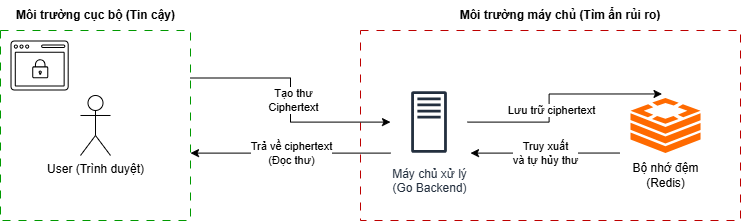
\includegraphics[width=\textwidth]{img/threat_model.png}
    \caption{Sơ đồ Luồng Dữ liệu (DFD) thể hiện Ranh giới Tin cậy (Trust Boundaries) trong kiến trúc Zero-Knowledge}
    \label{fig:threat_model_dfd}
\end{figure}

\textbf{Giả định cốt lõi về Ranh giới Tin cậy (Trust Boundary Assumption):} Mô hình đe dọa này được xây dựng dựa trên một giả thiết tối quan trọng: Trình duyệt web của người dùng (Client-side) phải là một môi trường an toàn và nguyên vẹn. Hệ thống Secret Letter không thể bảo vệ dữ liệu nếu bản thân thiết bị đã bị tổn hại từ trước (ví dụ: máy tính nhiễm mã độc, cài đặt các tiện ích mở rộng độc hại có khả năng đọc trộm bộ nhớ màn hình, hoặc hệ điều hành bị can thiệp). Đặc tính bảo mật đầu cuối chỉ phát huy tác dụng khi điểm cuối (Endpoint) thực sự nằm trong ranh giới an toàn.

\subsection{Spoofing (Giả mạo định danh)}

\textbf{Rủi ro:} Do đặc thù yêu cầu ẩn danh tuyệt đối, hệ thống chấp nhận rủi ro không thể xác thực danh tính người gửi (Spoofing) như một tính năng chủ đích (By-design). Tuy nhiên, kẻ tấn công có thể lợi dụng điều này để giả mạo hàng loạt người dùng nhằm phát tán thư rác (Spam) hoặc lạm dụng tài nguyên (Abuse).

\textbf{Biện pháp phòng ngừa:} Để ngăn chặn các cuộc tấn công lạm dụng, hệ thống triển khai cơ chế \textbf{Rate Limiting} nhiều lớp dựa trên địa chỉ IP (ví dụ: tạo tối đa 120 thư, giải mã 240 thư/giờ). Cần lưu ý sự đánh đổi (Trade-off): trong môi trường dùng chung IP (NAT) như trường học hoặc công ty, việc block IP có thể dẫn đến hiện tượng từ chối dịch vụ (DoS) cục bộ đối với các người dùng hợp lệ.

\subsection{Tampering (Can thiệp dữ liệu)}

\textbf{Rủi ro:} Kẻ tấn công, kể cả những quản trị viên có quyền truy cập vật lý vào cơ sở dữ liệu Redis, có thể cố tình chỉnh sửa nội dung bức thư (đã bị mã hóa) trước khi nó được gửi đến người nhận nhằm phá hoại tính toàn vẹn của dữ liệu.

\textbf{Biện pháp phòng ngừa:} Nhờ áp dụng thuật toán mã hóa \textbf{AES-256-GCM} (Galois/Counter Mode) cung cấp tính năng Authenticated Encryption, mọi nỗ lực thay đổi dù là một bit nhỏ nhất trên chuỗi \texttt{ciphertext} đều sẽ bị phát hiện trong quá trình giải mã tại trình duyệt. Cơ chế này đảm bảo nội dung thư nếu bị can thiệp sẽ hiển thị thông báo lỗi thay vì hiển thị dữ liệu sai lệch.

\subsection{Repudiation (Chối bỏ trách nhiệm)}

\textbf{Rủi ro:} Người gửi có thể phủ nhận việc đã gửi một bức thư có nội dung nhạy cảm, hoặc người nhận có thể phủ nhận việc đã đọc bức thư đó.

\textbf{Biện pháp phòng ngừa:} Rủi ro này thực chất được xem là một \textbf{tính năng} (Feature) của \textit{Secret Letter}. Dự án chủ trương thiết kế theo mô hình ẩn danh và không lưu vết (Anti-forensics). Hệ thống không lưu trữ địa chỉ IP, không ghi log thao tác cá nhân, và tự động hủy thư sau khi đọc. Do đó, việc không thể chứng minh ai là người gửi/người nhận là kết quả tất yếu của thiết kế Zero-Knowledge.

\subsection{Information Disclosure (Lộ lọt thông tin)}

\textbf{Rủi ro:} Nội dung bức thư có thể bị đánh cắp bởi tin tặc khi đang truyền tải trên mạng (Man-in-the-Middle) hoặc bị khai thác trực tiếp từ cơ sở dữ liệu máy chủ.

\textbf{Biện pháp phòng ngừa:} Đây là khía cạnh được hệ thống bảo vệ nghiêm ngặt nhất. Dữ liệu được bảo vệ bằng kênh truyền \textbf{TLS 1.3} chống nghe lén. Đột phá cốt lõi nằm ở kiến trúc \textbf{Client-Side Encryption (Mã hóa đầu cuối)}, trong đó khóa giải mã được truyền tải thông qua \textbf{URL Fragment} (\texttt{\#key}). Máy chủ chỉ nhận và lưu trữ bản mã vô nghĩa (\texttt{ciphertext}), hoàn toàn không có khả năng tự tiếp cận thông tin ngay cả khi bị tổn hại toàn diện.

\subsection{Denial of Service - DoS (Từ chối dịch vụ)}

\textbf{Rủi ro:} Hacker có thể liên tục gửi các yêu cầu tạo thư với Payload có kích thước khổng lồ nhằm làm cạn kiệt băng thông mạng, bộ nhớ RAM hoặc năng lực xử lý CPU của hệ thống.

\textbf{Biện pháp phòng ngừa:} Để chống lại các cuộc tấn công DoS, backend Golang được cấu hình với \texttt{http.MaxBytesReader} để ngắt kết nối ngay lập tức nếu dung lượng Request vượt quá giới hạn thiết kế. Đồng thời, cấu trúc dữ liệu trên Redis chia tách rõ ràng giữa Metadata (có kích thước cực nhỏ để truy vấn nhanh) và Payload, giúp hệ thống duy trì hiệu suất tra cứu ngay cả khi đang bị tấn công lưu lượng lớn.

\subsection{Elevation of Privilege (Nâng quyền hệ thống)}

\textbf{Rủi ro:} Kẻ tấn công có thể khai thác các lỗ hổng bảo mật trong mã nguồn Backend hoặc hệ điều hành để chiếm quyền điều khiển cao hơn, từ đó can thiệp vào tiến trình của ứng dụng.

\textbf{Biện pháp phòng ngừa:} Môi trường Backend được đóng gói bằng công nghệ Docker Container với tùy chọn \texttt{security\_opt: no-new-privileges:true} và giới hạn thư mục gốc ở chế độ \texttt{read\_only}. Việc thu hồi các quyền quản trị không cần thiết (Cap\_drop) giúp "giam lỏng" tiến trình ứng dụng, ngăn chặn khả năng kẻ tấn công vượt ngục (Container Escape) ra máy chủ vật lý.
\section{Chiến lược kiểm thử}
\section{Đánh giá hiệu năng}
\section{Quy trình CI/CD và Triển khai}
\label{sec:cicd_pipeline}

Để đảm bảo chất lượng mã nguồn và tự động hóa quy trình phân phối, dự án Secret Letter xây dựng luồng CI/CD (Continuous Integration / Continuous Deployment) hoàn chỉnh thông qua nền tảng \textbf{GitHub Actions}.

Sơ đồ \ref{fig:cicd_pipeline} minh họa tổng quan kiến trúc của hai luồng tự động hóa chính, đóng vai trò như những "chốt chặn chất lượng" (Quality Gates) trước khi đưa sản phẩm đến tay người dùng.

\begin{figure}[htbp]
    \centering
    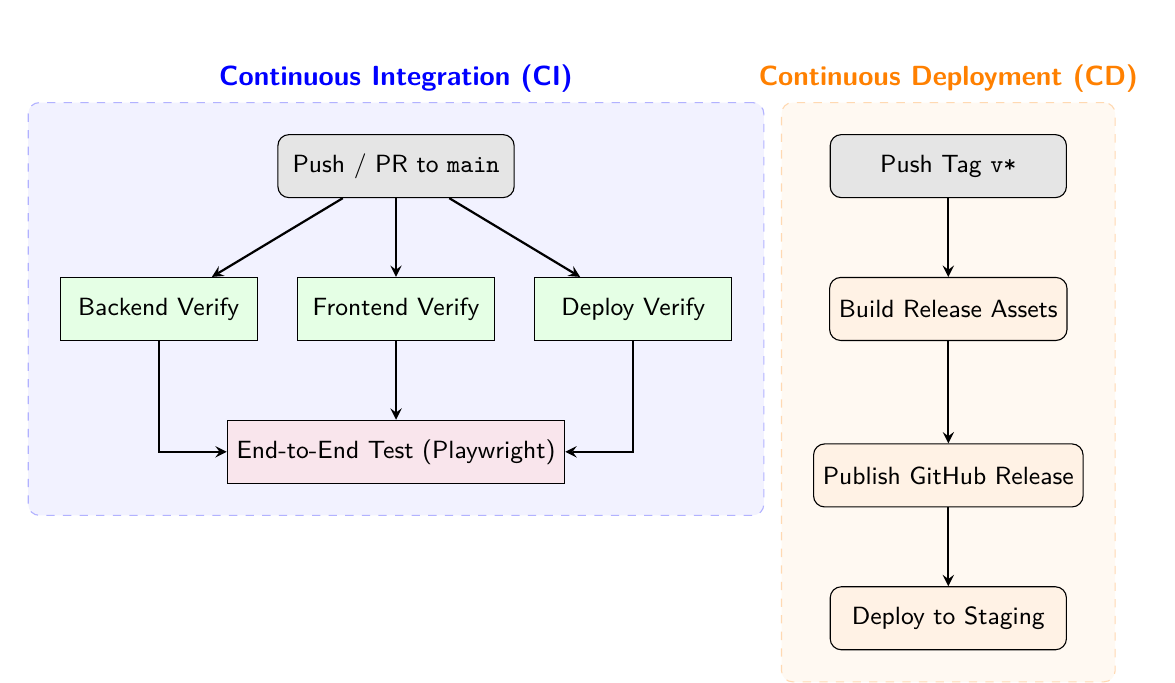
\begin{tikzpicture}[
        node distance=1.2cm and 1.2cm,
        box/.style={rectangle, draw, rounded corners, fill=gray!20, minimum width=3cm, minimum height=0.8cm, align=center, font=\sffamily\small},
        action/.style={rectangle, draw, fill=green!10, minimum width=2.5cm, minimum height=0.8cm, align=center, font=\sffamily\small},
        deploy/.style={rectangle, draw, rounded corners, fill=orange!10, minimum width=3cm, minimum height=0.8cm, align=center, font=\sffamily\small},
        arrow/.style={thick,->,>=stealth},
        line/.style={thick,-}
        ]
        
        % Nodes
        \node (push) [box] {Push / PR to \texttt{main}};
        
        \node (frontend) [action, below=1cm of push] {Frontend Verify};
        \node (backend) [action, left=0.5cm of frontend] {Backend Verify};
        \node (deployverify) [action, right=0.5cm of frontend] {Deploy Verify};
        
        \node (e2e) [action, below=1cm of frontend, fill=purple!10, minimum width=3cm] {End-to-End Test (Playwright)};
        
        \node (tag) [box, right=4cm of push] {Push Tag \texttt{v*}};
        
        \node (build) [deploy, below=1cm of tag] {Build Release Assets};
        \node (publish) [deploy, below=1.3cm of build] {Publish GitHub Release};
        \node (staging) [deploy, below=1cm of publish] {Deploy to Staging};
        
        % Background boxes
        \begin{scope}[on background layer]
            \node[fill=blue!5, rounded corners, draw=blue!30, dashed, fit=(push) (backend) (frontend) (deployverify) (e2e), inner sep=0.4cm, label={[font=\sffamily\bfseries, text=blue]above:Continuous Integration (CI)}] (ci_box) {};
            \node[fill=orange!5, rounded corners, draw=orange!30, dashed, fit=(tag) (build) (publish) (staging), inner sep=0.4cm, label={[font=\sffamily\bfseries, text=orange]above:Continuous Deployment (CD)}] (cd_box) {};
        \end{scope}

        % Arrows
        \draw [arrow] (push) -- (backend);
        \draw [arrow] (push) -- (frontend);
        \draw [arrow] (push) -- (deployverify);
        
        \draw [arrow] (backend) |- (e2e);
        \draw [arrow] (frontend) -- (e2e);
        \draw [arrow] (deployverify) |- (e2e);
        
        \draw [arrow] (tag) -- (build);
        \draw [arrow] (build) -- (publish);
        \draw [arrow] (publish) -- (staging);
        
    \end{tikzpicture}
    \caption{Sơ đồ tổng quan kiến trúc CI/CD bằng GitHub Actions}
    \label{fig:cicd_pipeline}
\end{figure}

\subsection{Giai đoạn 1: Tích hợp liên tục và Kiểm duyệt (CI)}
Luồng Tích hợp liên tục (CI) đóng vai trò là hàng rào bảo mật và kiểm thử cốt lõi. Cụ thể, thông qua tính năng \textbf{Branch Protection} của GitHub, nhánh \texttt{main} được khóa lại, yêu cầu bất kỳ đoạn mã mới nào (Pull Request) cũng phải vượt qua 100\% các bài test tự động trước khi được hợp nhất (Merge).

Luồng này bao gồm các công đoạn:
\begin{itemize}
    \item \textbf{Phân tích Tĩnh \& Unit Test:} Mã nguồn Backend được quét lỗ hổng bằng \texttt{gosec} (phát hiện rò rỉ mã hóa, SQL Injection) và \texttt{govulncheck} (quét các lỗ hổng CVE trong thư viện). Tại Frontend, các bài test được khởi chạy bằng \texttt{Jest} kết hợp với lệnh \texttt{npm audit} để loại trừ thư viện độc hại.
    \item \textbf{Tính Toàn vẹn cấu hình (Deploy Verify):} Hệ thống chạy môi trường giả lập nhằm biên dịch thử tệp \texttt{docker-compose} và \texttt{Caddyfile}, đồng thời sinh mã băm SHA256 giả lập để đảm bảo kịch bản bash shell không có lỗi cú pháp.
    \item \textbf{Kiểm thử Đầu - Cuối (End-to-End):} Sau khi các bước Unit Test hoàn tất, một phiên bản trình duyệt Chromium không giao diện (Headless) được \textbf{Playwright} khởi chạy để mô phỏng một luồng tạo thư và giải mã hoàn chỉnh của người dùng thực.
\end{itemize}

Sự kết hợp này đảm bảo tính năng mới không bao giờ làm hỏng kiến trúc Zero-Knowledge đã thiết kế ở Chương 3.

\subsection{Giai đoạn 2: Phát hành và Triển khai liên tục (CD)}
Luồng Triển khai (CD) chỉ được kích hoạt khi nhà phát triển đánh dấu một mốc phát hành (Tag \texttt{v*}). Lúc này, thay vì kiểm thử, GitHub Actions sẽ đóng vai trò như một cỗ máy biên dịch và phân phối:
\begin{itemize}
    \item \textbf{Đóng gói Tài nguyên (Build Assets):} Backend Go được biên dịch chéo (Cross-compile) thành tệp nhị phân cho Linux, trong khi Frontend được Vite đóng gói thành tài nguyên tĩnh. Một bản kê khai \texttt{release-manifest.json} chứa mã băm SHA256 của từng tệp được tạo ra để đảm bảo không có sự can thiệp từ bên thứ ba trong quá trình tải xuống.
    \item \textbf{Phân phối \& Triển khai:} Các tệp nén (\texttt{.tar.gz}) được đính kèm trực tiếp vào trang GitHub Release. Sau đó, máy chủ CI kết nối SSH an toàn vào VPS (môi trường Staging) thông qua \texttt{GitHub Secrets}, giải nén và cập nhật dịch vụ mà không yêu cầu can thiệp thủ công từ kỹ sư vận hành.
\end{itemize}
\newpage

\chapter*{KẾT LUẬN}
\addcontentsline{toc}{chapter}{KẾT LUẬN}

Dự án \textit{Secret Letter} đã hiện thực hóa một hệ thống truyền tải thông điệp nhạy cảm dựa trên nền tảng kiến trúc Zero-Knowledge. Bằng cách dịch chuyển trọng tâm xử lý mã hóa (thông qua Web Crypto API với thuật toán AES-GCM) về phía thiết bị đầu cuối, dự án đã thu hẹp đáng kể đặc quyền giám sát của máy chủ trung gian. Kết hợp với cơ chế tiêu hủy nguyên tử (Atomic Burn-after-reading) được kiểm soát bởi các kịch bản Lua trên hệ thống lưu trữ Redis, giải pháp kỹ thuật này đảm bảo dữ liệu chỉ có thể được trích xuất và giải mã một lần duy nhất bởi thực thể nắm giữ phân đoạn khóa (\texttt{\#key}).

Dưới góc nhìn kiến trúc phần mềm, mô hình trên phản ánh sự đánh đổi (trade-off) giữa độ an toàn và khả năng phục hồi (Recoverability). Việc máy chủ từ bỏ khả năng can thiệp vào bản rõ (Plaintext) đồng nghĩa với việc hệ thống không thể khôi phục dữ liệu khi người dùng đánh mất khóa mã hóa. Dù vậy, trước rủi ro rò rỉ dữ liệu (Data Breach) tại các điểm lưu trú tập trung, quyết định thiết kế này thiết lập một ranh giới bảo mật bằng kỹ thuật mật mã học thay vì chỉ dựa vào các chính sách cam kết quyền riêng tư (Privacy Policy).

Định hướng phát triển tiếp theo của dự án tập trung vào việc nghiên cứu áp dụng chứng minh không tiết lộ thông tin (Zero-Knowledge Proofs - ZKP) để xác thực danh tính người nhận mà không yêu cầu cung cấp thông tin cá nhân. Bên cạnh đó, việc đóng gói luồng xử lý mật mã tại Frontend thành các mô-đun WebAssembly (Wasm) là một hướng đi khả thi nhằm gia tăng độ khó đối với các nỗ lực dịch ngược mã nguồn (Reverse Engineering) từ phía kẻ tấn công.

\clearpage


\addcontentsline{toc}{chapter}{\textbf{TÀI LIỆU THAM KHẢO}}
\renewcommand{\bibname}{\centering \textbf{\fontsize{16pt}{18pt}\selectfont TÀI LIỆU THAM KHẢO}}

\printbibliography

% ==================== PHỤ LỤC (nếu có) ======================
% \newpage
% \appendix
% \renewcommand{\chaptername}{PHỤ LỤC} % Đổi tên CHƯƠNG thành PHỤ LỤC

% \chapter{CÁC ĐOẠN MÃ NGUỒN CỐT LÕI}

% 

% --- PHẦN A1 ---
\section*{A1. Sinh cặp khóa RSA bằng Web Crypto API: crypto.ts}

\begin{minted}[language=typescript, caption={Sinh cặp khóa RSA}, label={lst:gen-rsa-keypair}]{typescript}
export async function generateRSAKeyPair(): Promise<RSAKeyPair> {
    const keyPair = await crypto.subtle.generateKey(
        RSA_ALGORITHM,
        true, // extractable
        ["encrypt", "decrypt"]
    );

    return {
        publicKey: keyPair.publicKey,
        privateKey: keyPair.privateKey,
    };
}
\end{minted}

% --- PHẦN A2 ---
\section*{A2. Mã hóa AES-GCM + đóng gói (nonce + ciphertext + tag $\to$ Base64): crypto.ts}

\begin{minted}[language=typescript, caption={Hàm mã hóa AES-GCM}, label={lst:aes-encrypt}]{typescript}
export async function aesEncrypt(
    plaintext: string,
    aesKey: CryptoKey,
    additionalData?: BufferSource
): Promise<string> {
    const nonce = crypto.getRandomValues(new Uint8Array(NONCE_LENGTH));
    const plaintextBytes = stringToArrayBuffer(plaintext);

    const encryptParams: AesGcmParams = { name: "AES-GCM", iv: nonce };
    if (additionalData) {
        encryptParams.additionalData = additionalData;
    }

    const ciphertext = await crypto.subtle.encrypt(
        encryptParams,
        aesKey,
        plaintextBytes
    );

    const combined = new Uint8Array(nonce.length + ciphertext.byteLength);
    combined.set(nonce, 0);
    combined.set(new Uint8Array(ciphertext), nonce.length);

    return arrayBufferToBase64(combined.buffer);
}
\end{minted}

\noindent (đóng gói thông điệp khi gửi, gắn nhãn E2EE):

\begin{minted}[language=typescript, caption={Xử lý gửi tin nhắn có mã hóa}, label={lst:send-msg-logic}]{typescript}
const encryptResult = await encryptMessage(otherUser._id, currentValue.trim());
if (encryptResult) {
  const encryptedContent = `E2EE:${encryptResult.ciphertext}`;
  await sendDirectMessage(
    otherUser._id,
    encryptedContent,
    undefined,
    currentValue.trim(),
    encryptResult.counter
  );
}
\end{minted}

% --- PHẦN A3 ---
\section*{A3. Dẫn xuất khóa từ PIN bằng PBKDF2: crypto.ts}

\begin{minted}[language=typescript, caption={Dẫn xuất khóa AES từ PIN thông qua PBKDF2}, label={lst:derive-key-pin}]{typescript}
export async function deriveKeyFromPIN(
    pin: string,
    salt: Uint8Array,
    iterations: number = 100000
): Promise<CryptoKey> {
    const pinBuffer = stringToArrayBuffer(pin);

    const keyMaterial = await crypto.subtle.importKey(
        "raw",
        pinBuffer,
        "PBKDF2",
        false,
        ["deriveBits", "deriveKey"]
    );

    const derivedKey = await crypto.subtle.deriveKey(
        {
            name: "PBKDF2",
            salt,
            iterations,
            hash: "SHA-256",
        } as Pbkdf2Params,
        keyMaterial,
        {
            name: "AES-GCM",
            length: 256,
        },
        true,
        ["encrypt", "decrypt"],
    );

    return derivedKey;
}
\end{minted}

% --- PHẦN 4 ---
\section*{A4. Middleware/Dependency xác thực JWT: auth.py}

\begin{minted}[language=python, caption={Dependency lấy thông tin user hiện tại từ Token}, label={lst:backend-get-current-user}]{python}
security = HTTPBearer()

async def get_current_user(
    credentials: HTTPAuthorizationCredentials = Depends(security),
) -> User:
    try:
        token = credentials.credentials
        user_id = verify_access_token(token)

        if not user_id:
            raise credentials_exception

        user = await User.get(user_id)
        if user is None:
            raise credentials_exception

        return user
    except ValueError:
        raise credentials_exception
    except Exception as e:
        raise credentials_exception
\end{minted}

\noindent JWT verify nằm tại: \texttt{security.py}

\begin{minted}[language=python, caption={Hàm giải mã và kiểm tra JWT Token}, label={lst:backend-verify-token}]{python}
def verify_access_token(token: str) -> str:
    settings = get_settings()
    try:
        payload = jwt.decode(token, settings.secret_key,
                             algorithms=[settings.algorithm])
        return str(payload["sub"])
    except (KeyError, JWTError) as exc:
        raise ValueError("Invalid authentication token") from exc
\end{minted}

% --- PHẦN A5 ---
\section*{A5. WebSocket chuyển tiếp tin nhắn realtime (emit/broadcast): con\-nec\-tion\_ma\-na\-ger.py}

\begin{minted}[language=python, caption={Hàm phát tin nhắn tới client qua WebSocket}, label={lst:ws-emit-msg}]{python}
async def emit_new_message(
    self,
    conversation_id: str,
    message: dict,
    conversation_data: dict,
    unread_counts: dict,
    participant_ids: List[str] | None = None
) -> None:
    data = {
        "message": message,
        "conversation": conversation_data,
        "unreadCounts": unread_counts,
    }

    if participant_ids:
        for user_id in participant_ids:
            self.join_room(user_id, conversation_id)
            await self.send_to_user(user_id, "new-message", data)
    else:
        await self.broadcast_to_room(conversation_id, "new-message", data)
\end{minted}

\noindent Gọi emit khi lưu tin nhắn: \texttt{message\_service.py}

\begin{minted}[language=python, caption={Kích hoạt sự kiện WebSocket sau khi lưu tin nhắn}, label={lst:service-call-emit}]{python}
await manager.emit_new_message(
    conversation_id=str(conversation.id),
    message=self._format_message(message),
    conversation_data=await self._format_conversation_for_ws(
        conversation, include_full=is_new_conversation),
    unread_counts={str(k): v for k, v in conversation.unread_counts.items()},
    participant_ids=participant_ids
)
\end{minted}
% \newpage
% \chapter{CẤU TRÚC MỘT VÀI GÓI TIN}
% % --- B1 ---
% Sửa: thêm \_ để thoát ký tự, thêm \- vào giữa e2eeService để ngắt dòng
\section*{B1. PublicKeyRegister (POST /api/e2ee/keys/register): e2ee.py, e2eeSer\-vice.ts}

\begin{minted}[language=json, caption={PublicKeyRegister payload}, label={lst:publickey-register}]{json}
{
  "public_key": "BASE64_SPKI_RSA_PUBLIC_KEY",
  "fingerprint": "SHA256_FINGERPRINT",
  "device_id": "optional-device-id",
  "device_name": "optional-device-name"
}
\end{minted}

% --- B2 ---
\section*{B2. SessionKeyExchange (POST /api/e2ee/session/exchange): e2ee.py, e2eeSer\-vice.ts}

\begin{minted}[language=json, caption={SessionKeyExchange payload}, label={lst:session-key-exchange}]{json}
{
  "recipient_id": "USER_ID",
  "encrypted_session_key": "BASE64_ENCRYPTED_AES_KEY",
  "target_device_id": "optional-device-id",
  "conversation_id": "optional-conversation-id",
  "key_version": 2,
  "signature": "BASE64_RSA_PSS_SIGNATURE",
  "timestamp": 1736251234567
}
\end{minted}

% --- B3 ---
\section*{B3. PendingKeyEnvelope (GET /api/e2ee/pending-keys): e2ee.py, e2eeSer\-vice.ts}

\begin{minted}[language=json, caption={PendingKeyEnvelope payload}, label={lst:pending-key-envelope}]{json}
{
  "id": "PENDING_KEY_ID",
  "conversation_id": "optional-conversation-id",
  "recipient_user_id": "USER_ID",
  "recipient_device_id": "optional-device-id",
  "key_version": 2,
  "encrypted_session_key": "BASE64_ENCRYPTED_AES_KEY",
  "sender_user_id": "SENDER_ID",
  "signature": "BASE64_RSA_PSS_SIGNATURE",
  "timestamp": 1736251234567,
  "created_at": "2026-01-06T21:45:00Z"
}
\end{minted}

% --- B4 ---
\section*{B4. PendingKeyAck (POST /api/e2ee/pending-keys/ack): e2ee.py, e2eeSer\-vice.ts}

\begin{minted}[language=json, caption={PendingKeyAck payload}, label={lst:pending-key-ack}]{json}
{
  "ids": ["PENDING_KEY_ID_1", "PENDING_KEY_ID_2"]
}
\end{minted}

% --- B5 ---
% Sửa: websocket_router -> websocket\-\_router (cho phép ngắt dòng trước dấu _)
\section*{B5. WebSocketEnvelope (WS runtime): websocket\-\_router.py, connection\-\_manager.py}

\begin{minted}[language=json, caption={WebSocket envelope}, label={lst:ws-envelope}]{json}
{
  "event": "event-name",
  "data": {
    "any": "payload"
  }
}
\end{minted}

% --- B6 ---
% Sửa: api_e2ee -> api\-\_e2ee, dùng $\to$ cho mũi tên đẹp hơn
\section*{B6. WS session-key-exchange (server $\to$ client): api\-\_e2ee.py, websocket\-\_router.py}

\begin{minted}[language=json, caption={WS session-key-exchange payload}, label={lst:ws-session-key-exchange}]{json}
{
  "event": "session-key-exchange",
  "data": {
    "senderId": "SENDER_ID",
    "senderUsername": "alice",
    "senderDisplayName": "Alice",
    "encryptedSessionKey": "BASE64_ENCRYPTED_AES_KEY",
    "deviceId": "device-id",
    "recipientDeviceId": "device-id",
    "conversationId": "optional-conversation-id",
    "keyVersion": 2,
    "signature": "BASE64_RSA_PSS_SIGNATURE",
    "timestamp": 1736251234567
  }
}
\end{minted}

% --- B7 ---
\section*{B7. WS new-message (server $\to$ client): message\-\_service.py, connection\-\_manager.py}

\begin{minted}[language=json, caption={WS new-message payload}, label={lst:ws-new-message}]{json}
{
  "event": "new-message",
  "data": {
    "message": {
      "_id": "MESSAGE_ID",
      "conversationId": "CONVO_ID",
      "senderId": "USER_ID",
      "content": "E2EE:BASE64_CIPHERTEXT",
      "imgUrl": null,
      "createdAt": "2026-01-06T21:45:00Z",
      "keyVersion": 2,
      "counter": 12
    },
    "conversation": {
      "_id": "CONVO_ID",
      "type": "direct",
      "lastMessage": {
        "_id": "MESSAGE_ID",
        "content": "E2EE:BASE64_CIPHERTEXT",
        "senderId": "USER_ID",
        "createdAt": "2026-01-06T21:45:00Z",
        "counter": 12,
        "keyVersion": 2,
        "sender": {
          "_id": "USER_ID",
          "displayName": "",
          "avatarUrl": null
        }
      },
      "lastMessageAt": "2026-01-06T21:45:00Z",
      "createdAt": "2026-01-06T20:00:00Z",
      "updatedAt": "2026-01-06T21:45:00Z"
    },
    "unreadCounts": {
      "USER_ID": 1
    }
  }
}
\end{minted}

\end{document}